%%%%%%%%%%%%%%%%%%%%%%%%%%%%%%%%%%%%%%%%%
% SC Information Paper 5 
% SHARK INDICATORS IN THE WESTERN CENTRAL PACIFIC
% June 2015
%
% Author: Joel Rice (joelrice@uw.edu )
%
%
%%%%%%%%%%%%%%%%%%%%%%%%%%%%%%%%%%%%%%%%%

%----------------------------------------------------------------------------------------
%  PACKAGES AND OTHER DOCUMENT CONFIGURATIONS
%----------------------------------------------------------------------------------------
\documentclass[12pt]{SCreport}

\graphicspath{ {C:/Projects/SHK-indicators-2015/GRAPHICS/} {C:/Projects/SHK-indicators-2015/GRAPHICS/Defined/} {C:/Projects/SHK-indicators-2015/GRAPHICS/CPUE_std/} }

\usepackage[english]{babel}
\usepackage{subfigure}
\newtoggle{includefigs}
%\togglefalse{includefigs} % to include figures, uncomment 
\toggletrue{includefigs}
\usepackage{graphicx}
\usepackage{multirow}
\usepackage{array}


  \reportauthor{Joel Rice\footnote{Joel Rice Consulting Ltd.}, Laura Tremblay-Boyer, and Shelton Harley}
  \reporttitle{Analysis of stock status and related indicators for key shark species of the Western Central Pacific Fisheries Commission}
  \reportnumber{SA-IP-05}



%----------------------------------------------------------------------------------------
%  Document content
%----------------------------------------------------------------------------------------

\begin{document}

\wcpfctitlepage

\tableofcontents

%\section{Executive Summary}

\section{Introduction} % ltb rev 90% done


% This study provides indicators related to the stocks general trend, whether it has changed from the previous indicator analysis and if further analysis is warrented, how to undertake that analysis.  Uncertainty regarding any species population level mechanisims that drive any indivudal anlysis is qualitiatively expressed  by species and stock in order to represent the uncertainty in the underlying data. 

Sharks are typically caught as bycatch in the Pacific tuna fisheries, though some directed and/or mixed species fisheries also exist. The status of the shark species designated as key shark species in 2011 (blue, mako, thresher, silky oceanic whiteip  sharks) in the western and central Pacific Ocean (WCPO) \hl{ADD REF} underwent a comprehensive review in 2011 \citep{Clarke2011_a}. This review presented a number of indicators to inform on the status of the stock of these shark species and their response to fishing pressure. Given the paucity of data availability for shark species compared to target species, these indicators were developed around the type of information typically available from operational-level data for industrial purse-seine and longline fleets. 

The current study updates key indicators and extends previous analyses to include hammerhead, porbeagle and \hlam{whale sharks}.  

We present information on the geographic range of catches for each of the species considered; temporal trends in catch composition and catch rates, and key biological indicators of fishing pressure such as mean size and sex ratio by species. Whale sharks are assessed separately due to the unique nature of their interactions with fisheries in the WCPO. The analyses are based on Secretariat of the Pacific Community - Oceanic Fisheries Programme (SPC-OFP) data holdings for sharks taken in longline and purse seine fisheries in the Western and Central Pacific Ocean (WCPO). The framework for the analysis is a series of indicators of fishing pressure and stock status that were first described in the Shark Research Plan presented to the sixth meeting of the Western and Central Pacific Fisheries Commission's (WCPFC) Scientific Committee (SC6; Clarke and Harley 2010). A preliminary indicator-based analysis of SPC data holdings was presented to the Commission in December 2010 (Clarke et al. 2010) with an exhaustive review of the fisheries and data sources presented to SC7 (Clarke et al. 2011). \hlcoral{end of this paragraph repeats first paragraph, need to merge}

\begin{comment}
Sharks are typically caught as bycatch in the Pacific tuna fisheries, though some directed and/or mixed species fisheries also exist. The status of the shark species designated as key shark species (blue, mako, thresher, silky and oceanic white tip sharks) in the western and central Pacific Ocean (WCPO) \hl{ADD REF} underwent a comprehensive review in 2011 \citep{Clarke2011_a}. Drawing on \citep{...}, this review presented a number of indicators to inform on the status of the stock of these shark species and their response to fishing pressure. Given the paucity of data availability for shark species compared to target species, these indicators were developed around the type of information typically available from operational-level data for industrial purse-seine and longline fleets. 

The current study updates key indicators and extends the analyses to include hammerhead, porbeagle and whale sharks. We present information on the geographic range of catches for each of the species considered; temporal trends in catch composition and catch rates, and key biological indicators of fishing pressure such as mean size and sex ratio by species. Whale sharks are assessed separately due to the unique nature of their interactions with fisheries in the WCPO. The analyses are based on Secretariat of the Pacific Community - Oceanic Fisheries Programme (SPC-OFP) data holdings for sharks taken in longline and purse seine fisheries in the Western and Central Pacific Ocean (WCPO). The framework for the analysis is a series of indicators of fishing pressure and stock status that were first described in the Shark Research Plan presented to the sixth meeting of the Western and Central Pacific Fisheries Commission's (WCPFC) Scientific Committee (SC6; Clarke and Harley 2010). A preliminary indicator-based analysis of SPC data holdings was presented to the Commission in December 2010 (Clarke et al. 2010) with an exhaustive review of the fisheries and data sources presented to SC7 (Clarke et al. 2011). \hlcoral{end of this paragraph repeats first paragraph, need to merge}
\end{comment}

\subsection{Report layout}
This report is necessarily large. To assist the reader it has been structured along the following lines. Following a brief description of the available data in section 2, each of the four indicator analyses are described and results summarized in section 3. Section 4 presents a consideration of the feasibility of conducting a formal stock assessment for each of the shark species discussed in this report.  In Section 5, we review the impact of recent shark management measures and, in section 6, recommend future work to extend and improve the indicator analysis approach.  Finally, section 7 discusses the management implications arising from the results of the work presented here.

\section{Description of Data}

The primary source of catch information regarding sharks is the SPC-held observer database which, despite low coverage in all regions (Table 1 \%Observer coverage by region), has a substantial amount of information regarding operational characteristics as well as fate and condition data on captured sharks. Observed hooks set is used here because it is a "common currency" and allows for the standardisation of observer coverage rates when undertaking analyses.  In addition to the observer data, SPC holds operational logsheet and aggregate data on shark catches by longline fisheries. The operational data submitted to the SPC are at a higher spatial resolution than the aggregate data, and are useful for catch estimation, but in practice their utility is limited by the lack of data provision by species for shark (Table 2 Logsheet coverage by region \% that ID sharks to species), especially in equatorial regions where the majority of the longline effort occurs. 
This study covers the time period 1995-2014, while while some observer and logbook data exist for years prior to 1995, the majority of records either do not report shark or list it as a general category 'shark'.  At the time of analysis sufficient data for 2014 was available both in logsheets and the observer data, notable exceptions from the observer database for  2014 are Australia and the United States whose most recent contributions was 2011.
%JR
%The primary source of catch information regarding sharks is the SPC held observer data which, despite low coverage in all regions (Table 1 -\%Observer coverage by region) has a significant amount of information regarding operational characteristics as well as the fate and condition of sharks caught. In addition to the observer data, SPC holds operational logsheet and aggregate data on shark catches by longline fisheries. The operational data submitted to the SPC are at a higher spatial resolution, and are useful for catch estimation, but in practice the utility is limited by the lack of data provision by species for shark \hl{(Table 2 Logsheet coverage by region \% that ID sharks to species)}, especially in equatorial regions where the majority of the longline effort occurs
%(\ref{fig:regions}).

Aggregate coverage rates are on par with the coverage rates of the operational logsheet data sets, although coverage differs greatly by region (Table 3). Historical coverage rates are poor partly because prior to February 2011 sharks were not amongst the species for which data provision was required (WCPFC 2013); since that time, data provision for the 13 species designated by WCPFC as key shark species is mandatory . Under CMM 2007-01, required levels of Regional Observer Programme (ROP) coverage in longline fisheries are set to rise to 5\% from June 2012 in most areas, but annual average values have been <1\% in recent years (for the entire WCPO). With some notable exceptions (e.g. northeast and southwest of Hawaii), most observed sets occurred within Exclusive Economic Zones (EEZs). A thorough examination of the SPC-held fisheries data and its utility for shark related analyses can be found in Clarke et al. (2011).

Building on the work of Clarke et al (2011), this indicator analysis uses the six WCPFC statistical areas as defined in the 2010 WCPFC bigeye tuna stock assessment (Figure 1). As noted in Clarke et al. (2011), these regions are somewhat arbitrarily assigned to the key shark species. However, given the fact that the predominant source of fishing mortality for these species is the longline fishery targeting tropical tunas (as well as billfishes and occasionally sharks), these regions adequately capture the important characteristics of the fisheries. Therefore, for purposes of comprehension and comparison to the previous analysis, we opted to keep the same regions. \hllb{Mention that current BET stock assessment uses different region and that the current set also captures key pattern like eastern end of Japanese fleet for region 1.}


%\addcenterfig]{}{P}

\begin{figure}
\begin{center}
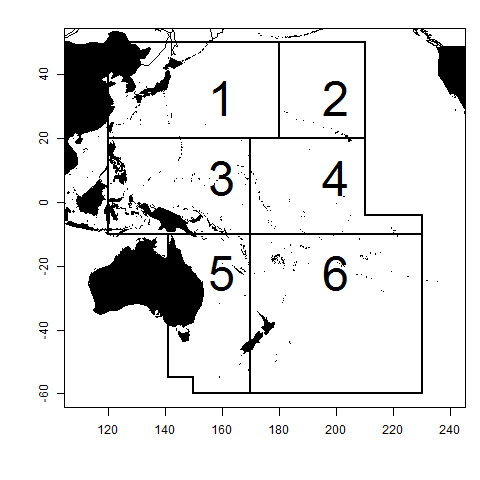
\includegraphics[scale=0.95]{../GRAPHICS/Defined/FIG_01_MAP}
\caption{\label{fig:regions} Map of WCPO and regions used for the analysis.}
\end{center}
\end{figure}

%----------------------------------------------------------------------------------------

\subsection{Longline Fishery Data}
%---------------------------------------------------------------------------------------------
\hllb{Put this somewhere: With the exception of 2014 total effort in the longline fleet has increased, througout the study  period (1995-2014) to approximately 800 million hooks annually with nearly half occuring in regions 3 and 4.}
  
  
Ideally, indicator analyses would be based on operational-level data as its higher spatial resolution permits more comprehensive and nuanced analyses, however SPC's operational level data is geographically limited with respect to provision of shark data.  Figure 2 illustrates the geographic distribution of sets for which SPC holds operational data (blue dots) and sets with at least one recorded shark are overplotted (in orange). However, this picture is somewhat misleading as only 41\% of the operational-level sets plotted recorded any sharks. This is in contrast to the observer data in which 93\% of the sets recorded at least one shark (overplotted in red).

This is not necessarily due to misreporting. Prior to February 2011, sharks were not amongst the species for which data provision was required (WCPFC 2011); since that time data provision for the 13 species designated by WCPFC as key shark species has been mandatory. Figure 2 does not distinguish between key shark species and other shark species because only 16\% of the reported sets recorded any species-specific shark catches. Clarke et al. (2011b) note that most historical species-specific shark catch data are provided by a small number of flag States.

Given the relatively low level of coverage in the operational-level logsheets, a more complete characterization of the longline fishery requires the use of the SPC-held aggregated (5x5 degree grid) data. Effort and reported shark catch data by flag at the aggregated level have a lower degree of spatial resolution but in most cases are raised to represent the entire WCPO longline fishery. Sets with observers present onboard, are shown for comparison (Figure 3) but have a finer degree of spatial resolution due to observer record keeping. Following CMM 2007-01, required levels of Regional Observer Programme (ROP) coverage in longline fisheries were set to rise to 5\% in June 2012 but annual average values have been on the order of 1-2\%.

A comparison of longline effort by flag and the number of sharks recorded in logsheets was constructed (\hllb{Figure 4}) by showing the top four fishing nations (in the WCPO as a whole) and aggregating the rest of the flag states to another group. If the fishing practices and reporting practices were more or less consistent across flags the numbers of sharks reported would be proportional, by flag, to the effort.

Comprehensive data on shark catches at high spatial resolution are available from observer data held by the SPC-OFP but, as described above, the overall coverage of these data is low, and less than the required levels of ROP coverage. In addition, a comparison of longline effort and longline observer coverage (\hllb{Figure 5}) reveals that the latter is disproportional by region and flag and thus cannot be considered representative of the fishery as whole.

Another aspect of the low data coverage problem is that of temporal representativeness on a month/year basis of the observed effort. A comparison of the annual proportion observed by month - on a regional basis - shows significant fluctuations in the relative coverage of the observer data compared to the logbook data (\hllb{Figure 6}).

\begin{comment}
%\hl{ SPC holds logsheet data on shark catches by longline fisheries at the operational and aggregate levels. Due to its higher spatial resolution, operational-level data would in theory be preferred for indicator analysis but in this case its geographic coverage is limited due to lack of data provision with respect to shark catches.  
%Sets for which at least one shark of any type was recorded in operational-level logsheet data held by SPC-OFP are distributed widely throughout the study area (%\ref{fig:LLsets}
%red points).}
%However, this picture is somewhat misleading due to overplotting as only

% 41\% of the operational-level sets plotted recorded any sharks. This is in contrast to the observer data in which 93\% of the sets recorded at least one shark.
  % load( file= "C:/Projects/SHK-indicators-2015/DATA/ll_obs_set_with_HW_11JUNE2015.rdata"  ) # loads shk_all  # 
  %  head(shk_all) 
  %  shk_all$comb_shk <- rowSums( shk_all[,c('totalshk', "othershk") ]  )
  %  temp<- with(shk_all, table(comb_shk>0)); obs_pos <- temp[2]/nrow(shk_all)
  %  print(paste(round(100*obs_pos), "% of observed sets recorded sharks"))
  % "93 % of observed sets recorded sharks"
   
%This is not necessarily due to miss reporting, wheras prior to February 2011 sharks were not amongst the species for which data provision was required (WCPFC 2011); since that time data provision for the 13 species designated by WCPFC as key shark species is mandatory. This plot does not distinguish between key shark species and other shark species because only  16\%
 %   shkLLlog$species_specific <- rowSums(shkLLlog[,c(36:69, 71)] )
 %   temp<-   with(shkLLlog, table(shkLLlog$species_specific>0)); log_sspec <- temp[2]/nrow(shkLLlog)
 %   print(paste(round(100*log_sspec), "% of operational sets recorded species specific shark "))
 %   16 % of operational sets recorded species specific shark "
%   of the reported sets recorded any species-specific shark catches. Clarke et al ( 2011b) note that most historical species-specific shark catch data are provided by a small number of flag States (Clarke et al 2011b).


Given the relatively low level of coverage in the operational-level logsheets, a more complete characterization of the longline fishery requires the use of aggregated (5x5 degree grid) data. Effort and reported shark catch data by flag at the aggregated level have a lower degree of spatial resolution but in most cases are raised to represent the entire WCPO longline fishery (Figures 3 and 4). Sets with observer present onboard, are shown for comparison but have a finer degree of spatial resolution due to observer record keeping. The observer data were plotted in red on the 
%\ref{fig:LLsets}.
Under CMM 2007-01, required levels of Regional Observer Programme (ROP) coverage in longline fisheries are set to rise to 5\% in June 2012 but annual average values have been on the order of 1\%-2\%.
% 
%  load( file= "C:/Projects/SHK-indicators-2015/DATA/ll_obs_set_with_HW_11JUNE2015.rdata"  ) # loads shk_all  # 
%      obshook <- with(shk_all, tapply(hook_est, list(yy,region), sum) )
%  load( file= "C:/Projects/SHK-indicators-2015/DATA/agg_eff_by_flag.rdata"  ) # loads shk_all  # 
%    fishhook  <-  with(aggr, tapply(hhooks, list(yy,region), sum) )
%   pcntobs <- obshook/(fishhook*100)
%   matplot(rownames(pcntobs),100* pcntobs, type='b', pch=as.character(1:6), col=rainbow(6), lty=1, bg="grey",lwd=2, ylab="Percentage Observer Coverage", las=1)
%  
%  annual_coverage <- round(100* with(shk_all, tapply(hook_est, list( yy), sum) )/(100*with(aggr, tapply(hhooks, list(yy ), sum) )), 2)
%  1995 1996 1997 1998 1999 2000 2001 2002 2003 2004 2005 2006 2007 2008 2009 2010 2011 2012 2013 2014 
%  0.48 0.50 0.63 0.51 0.41 0.71 1.13 1.72 1.74 1.69 1.48 1.60 1.45 1.27 1.13 1.05 1.00 0.22 0.90 0.75 
% all straight from the previous papers...


A comparison of longline effort by flad and the number of sharks recorded in logsheets was constructed by showing the top four fishing nations (in the WCPO as a whole) and aggregating the  rest of the flag states to an other group. If the fishing practices and reporting practices were more or less consistent across flags the  numbers of sharks reported would be proportional, by flag, to the effort.   

%\addcenterfig[Total number of hooks fished by flag (for the top four fishing nations, and all others combined) based on   aggregated (5x5 degree square) data, for six regions of the WCPFC Statistical Area. ]{fig:LLLogbood_flag_hooks}{FIG_xx_LLeff_FLAG}
%Comparison by region and flag of longline logsheet effort (left panel, in hundreds of hooks) and total sharks recorded on logsheets (right panel, in number of sharks), using aggregated (5x5 degree square) data, for six regions of the WCPFC Statistical Area


%\addcenterfig[Total number of reported sharks  by flag (for the top four fishing nations, and all others combined) based aggregated (5x5 degree square) data, for six regions of the WCPFC Statistical Area.]{fig:LLLog_flag_shks}{FIG_xx_LLreported_catch_FLAG}

Comprehensive data on shark catches at high spatial resolution are available from observer data held by the SPC-OFP but, as described above, the overall coverage of these data is low, and less than the required levels of  ROP  coverage. In addition, a comparison of longline effort  
%\ref{fig:LLLogbood_flag_hooks}
and longline observer coverage
%\ref{fig:obsLL_flag}
reveals that the latter is disproportional by region and flag and thus cannot be considered representative of the fishery as whole. 

%\addcenterfig[Total number of hooks observed by flag (for the top four fishing nations) based on longline observer records held by the SPC-OFP, for six regions of the WCPFC Statistical Area  ]{fig:obsLL_flag}{FIG_xx_LLeff_obs_FLAG}   

Another aspect of the low data coverage problem is that a temporal representativeness on a month/year basis of the  the observed effort 
%\ref{fig:obseffmnth} in comparison to the logsheet data
%\ref{logeffmnth}.
A comparison of the  annual  proportion observed by month - on a regional basis - shows significant fluctuations in the relative coverage of the observer data compared to the logbook data %\ref{fig:effdiff}.  
\end{comment}
%\addcenterfig[Map of WCPO and observed effort. ]{fig:LLsets}{FIG_02_MAP_sets}

\begin{figure}
\begin{center}
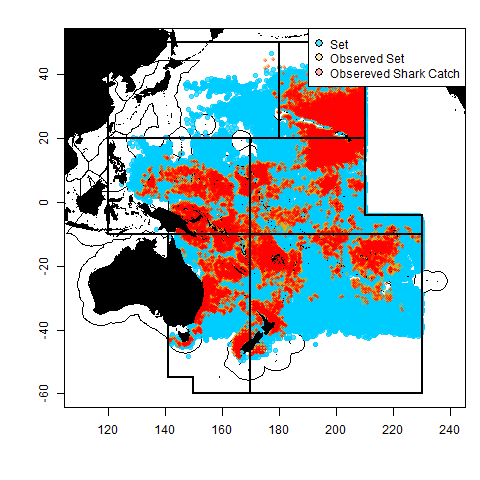
\includegraphics[scale=0.95]{../GRAPHICS/Defined/FIG_02_MAP_sets}
\caption{\label{fig:regions} Map of WCPO and observed effort.}
\end{center}
\end{figure}

\begin{figure}
\begin{center}
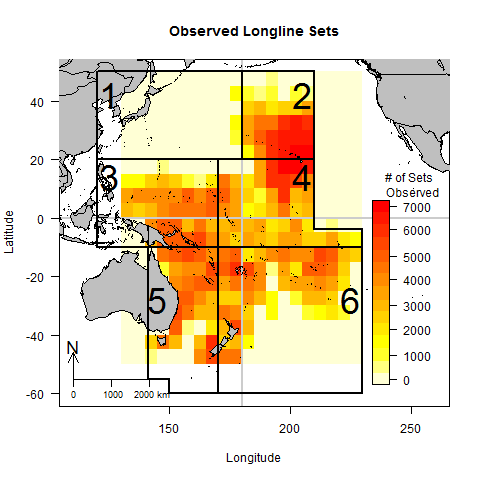
\includegraphics[scale=0.95]{../GRAPHICS/Defined/FIG_03_obs_ll_sets}
\caption{\label{fig:regions} Longline observed sets by 5x5 square}
\end{center}
\end{figure}


\begin{figure}
\centering
   \begin{subfigure}[b]{0.2\textwidth}
       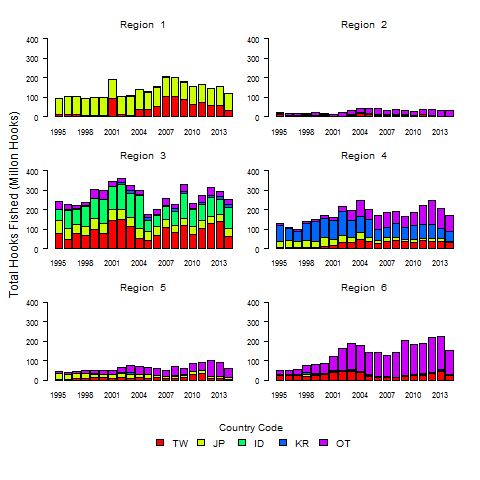
\includegraphics[width=\textwidth]{../GRAPHICS/Defined/FIG_04a_LLeff_FLAG_RDS}
%       \caption{CPUE(lb/hr) by fleet.}
%       \label{fig:Guam_cpue}
   \end{subfigure}
   \begin{subfigure}[b]{0.2\textwidth}
       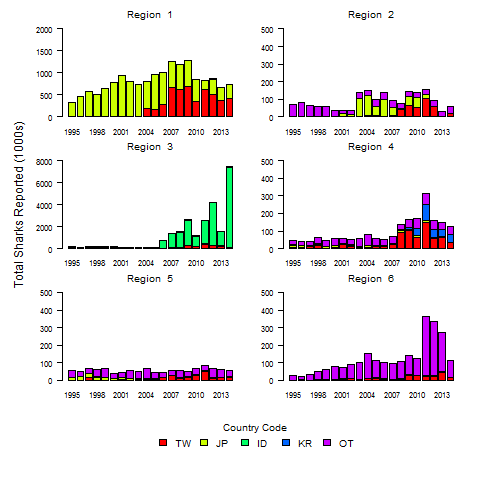
\includegraphics[width=\textwidth]{../GRAPHICS/Defined/FIG_04b_LLreported_catch_FLAG_RDS}
%       \caption{CPUE (fish/hr) fleets combined.}
%       \label{fig:Guam_creelcpue}
   \end{subfigure}
\caption{Estimated skipjack quarterly CPUE from the Guam troll fleets}\label{fig:Guam cpue}
\end{figure}


%\addcenterfig[Logsheet effort by month.]{fig:logeffmnth}{}
%\addcenterfig[Observed effort by month.]{fig:obseffmnth}{FIG_xx_obsBY_mm}
%\addcenterfig[Absolute percent difference in effort between reported (logsheet)  effort and observed effort.]{fig:effdiff}{FIG_xx_obsDIFFlog_mm}

\clearpage
%\addcenterfig[Aggregate effort by region. ]{fig:aggeff}{FIG_xx_agg_eff}
 
%-------------------------------------------------------------------------------------------------------------------------
 
 \subsection{Purse Seine data} 
 %N.B. all the stats quoted here are in PS_oper_stats.r (JR)
Similar to the longline fishery, SPC-OFP holds logsheet data on shark catches by purse seine fisheries at both the operational and aggregate levels.  However, operational-level coverage for the purse seine fishery (87\%) is considerably higher than for the longline fishery (23\%). This factor, in combination with the more limited geographic range of the purse seine fishery, contributes to more representative operation-level coverage in the purse seine fishery than in the longline fishery.

Following implementation of the WCPFC ROP on 1 January 2010, in combination with prior observer coverage commitments by Parties to the Nauru agreement (PNA) members, 100\% purse seine observer coverage is now required (except for vessels fishing exclusively in one Exclusive Economic Zone (EEZ)). Historical observer coverage in the purse seine fishery has varied between EEZs. Coverage rates were low, generally less than 10\%, for the years 1995-2002, with coverage increasing to 10-18\% for the years 2003-2009. Recent (2010-2013) annual averages are between 42-56\% in total.


While observer coverage of the purse seine fishery is not uniformly representative (Figure 7, orange points), it is more representative than observer coverage of the longline fishery, owing to both higher coverage levels and the more limited geographic range of the fishery (Lawson 2011). Regions 3 and 4 contain 98\% of the operational-level reported purse seine sets, and 99\% of observed sets and are thus the only regions for which purse seine analyses will be meaningful. Shark interactions are recorded in just 2.5\% of purse-seine operational logsheets (Figure 7, red points), a value far lower than the 41\% recorded in longline operational-level logsheet. As a result, it is not possible to assess the number of shark interactions by set or the species involved using purse seine logsheet data.

A comparison by flag of purse seine effort and the number of purse seine sets reporting at least one shark interaction was constructed for associated (floating object) and unassociated (free-swimming) sets based on aggregated logsheet data (Figure 8).  For each panel, flags were ranked by number of sets and the top four flags were plotted separately with all remaining flags aggregated into an "Other" category. Although estimated shark catches in the purse seine fishery are considerably lower than shark catches in the longline fishery (SPC 2008, Lawson 2011), it would still be expected that purse seine shark interactions are proportional to purse seine effort. However, from the discrepancies observed between the left and right panels, it appears that some major fishing nations are not submitting or are under-reporting their shark interactions.

\begin{figure}
\begin{center}
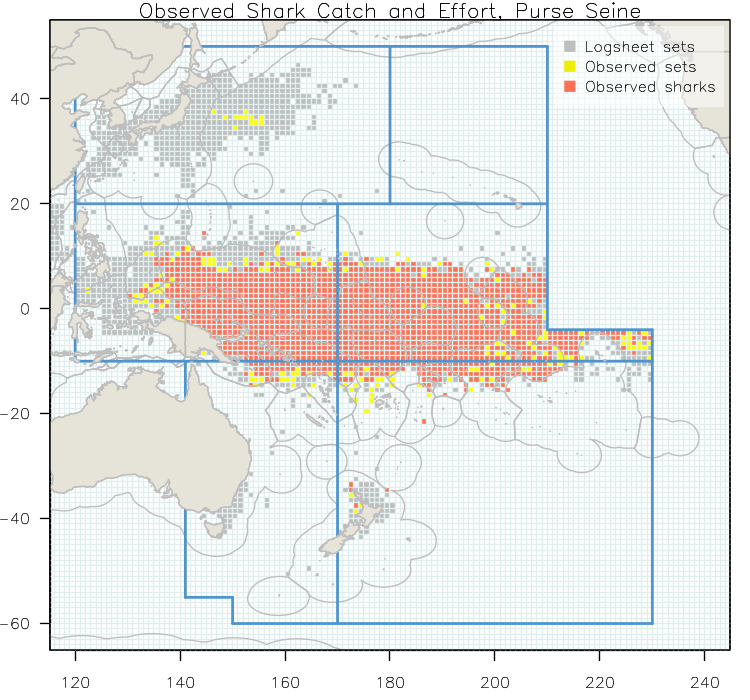
\includegraphics[scale=0.75]{../GRAPHICS/Defined/FIG_07_PS_sets}
\caption{\label{fig:regions} Absolute percent difference in effort between reported (logsheet)  effort and observed effort.}
\end{center}
\end{figure}

%  \addcenterfig[Absolute percent difference in effort between reported (logsheet)  effort and observed effort.]{fig:seine_map}{FIG_07_PS_sets}
 
 % old JR version 
 \begin{comment}
\hl{ As for the longline fishery, SPC-OFP holds logsheet data on shark catches by purse seine fisheries at the operational and aggregate levels, but operational-level coverage for the purse seine fishery,}
(87\%)  is considerably higher than for the longline fishery (23\%)
% sum(as.numeric( shklog$hook))/ sum(aggr$hhooks *100)
% print(paste0( "the operational level coverage of LL is ", round( 100* sum(as.numeric( shklog$hook))/ sum(aggr$hhooks *100),2   )))
% #"the operational level coverage of LL is 23.69"

This factor, in combination with the more limited geographic range of the purse seine fishery, contributes to more representative operation-level coverage in the purse seine fishery( \ref{fig:seine_map}  ) than in the longline fishery.

%\addcenterfig[Observed purse seine in the  WCPO showing the top four fishing nations and all others combined.  ]{fig:pssets}{FIG_xx_PS_eMAP_sets}


With implementation of the WCPFC ROP on 1 January 2010, in combination with prior observer coverage commitments by Parties to the Nauru Agreement (PNA) members, 100\% purse seine observer coverage is now required (except for vessels fishing exclusively in one exclusive economic zone (EEZ). Historical observer coverage in the purse seine fishery has varied between EEZs. Coverage rates were low, generally less than 10\% , for the years 1995-2002, with coverage incresing to 10-18\% for the years 2003-2009.  Recent  (2010-2013) annual averages are between 42-56\% in total. \hl{Although observer coverage of the purse seine fishery is not perfectly representative (Figure 2, orange points), the higher coverage levels and the more limited geographic range of the fishery result in more representative observer coverage for purse seines than for longlines (Lawson 2011 (Appendix Figure A2)). Regions 3 and 4 contain 98\% of the operational-level reported purse seine sets, and 99\% of observed sets and are thus the only regions for which purse seine analyses will be meaningful. In contrast to the longline operational-level logsheet data in which 41\% of recorded sets reported at least one shark}, only 2.5\% 
of purse seine operational-level logsheet sets reported any shark interactions (Figure \ref{fig:seine_map}, blue points). Due to inconsistent recording practices it is not possible to assess the number of shark interactions by set or the species involved using purse seine logsheet data.  

\hl{A comparison by flag of purse seine effort and the number of purse seine sets reporting at least one shark interaction was constructed for associated (floating object) and unassociated (free-swimming) sets based on aggregated logsheet data }
%Figure~\ref{fig:log_una_shk} \& Figure~\ref{fig:log_ass_shk}.

% note can we put the effort side by side with the shark reporting?
%  \addcenterfig[Comparison by region and flag of purse seine effort (in sets) associated sets using aggregated (5x5 degree square) data for six regions of the WCPFC Statistical Area, excluding data from Indonesia, Vietnam, and Japan coastal waters.]{fig:ps_ass_eff}{ps_total_effAssociated}
%   \addcenterfig[Comparison by region and flag of purse seine effort (in sets) unassociated sets using aggregated (5x5 degree square) data for six regions of the WCPFC Statistical Area, excluding data from Indonesia, Vietnam, and Japan coastal waters.]{fig:ps_una_eff}{ps_total_effUnassociated} 

%  \addcenterfig[Total sharks recorded on logsheets (in number of sets recording at least one shark interaction), for associated sets.]{fig:log_ass_shk}{ps_oper_shks_rep_cntry_associated}
%  \addcenterfig[Total sharks recorded on logsheets (in number of sets recording at least one shark interaction), for unassociated sets.]{fig:log_una_shk}{ps_oper_shks_rep_cntry_unassociated} 

For each panel, flags were ranked by number of sets and the top four flags were plotted separately with all remaining flags aggregated into an "Other" category.
Although estimated shark catches in the purse seine fishery are considerably lower than shark catches in the longline fishery (SPC 2008, Lawson 2011), it would still be expected that purse seine shark interactions are proportional to purse seine effort. However, from the discrepancies observed between the left and right panels in 
%Figure~\ref{fig:log_una_shk}
, it appears that some major fishing nations are not submitting or are under-reporting their shark interactions.
\end{comment} 
\clearpage         
 %       \subsection{Data formatting}
 %       \subsection{Limitations - Caveats}
        
        
%----------------------------------------------------------------------------------------
%  Distribuion Indicators
%----------------------------------------------------------------------------------------
             
        
\section{Distribution Indicator Analyses}
      \subsection{Introduction}

      Distribution indicators consider patterns in the geographic distribution of species catch. Spatial trends in fisheries data need to be interpreted carefully since they originate from a biased sampling design \citep{Walters2003_a}. If assessed carefully, however, they can provide useful insight into spatial and temporal trends in species distribution as well as highlight areas of strong interactions between a species and fisheries. In addition, changes in stock abundance might be reflected in distribution \citep{MacCall1990}, with increases and decreases in abundance resulting in range expansions and contractions, respectively. Such patterns have been reviewed at length in the terrestrial literature \citep{Borregaard2010_a} but less often for marine applications due to the paucity of historical data \citep[but see][]{Worm2011_a}. \hllb{FIX. The indicators presented below are based on observer data and thus patterns in fishing effort and/or observer coverage may bias the results.  These results should therefore be taken as an initial indication of the location and intensity of interactions between these species and WCPO longline fisheries.  They can be updated over time to determine if the spatial patterns change or temporal trends develop.  More complex methodologies might also be applied to remove potential sampling biases.}
      
\hllb{Potentially need to add back some of these.}\hl{These indicators examine the geographic range of each species and the habitat usage (in terms of geography only; oceanographic variables are not considered) by different life stages (adult/juvenile) and sexes based on fishery interaction data. Spatial analysis of fish occurrences can be useful in identifying range contractions or expansions which may be linked to fishing activities (Worm and Tittensor 2011). In addition, since many pelagic shark species are known to exhibit sex- and age- specific distribution patterns (Camhi et al. 2008, Mucientes et al. 2009) spatial analysis can highlight areas which are important to key life stages (e.g. presence of adult females and juveniles may indicate pupping grounds; presence of juveniles only may indicate nursery grounds).}
      
      
      \subsection{Methods}
      In this study, we calculated four Distribution Indicators:
      
\begin{itemize}
\item	Species-occurrence.  This indicator summarizes the occurrence of a species in any longline set monitored by an observer.  A positive value at any given location simply indicates that the species in question was observed at least once, without regard to annual frequency or fishing effort.

\item	Proportion-presence.  This indicator provides a rough indicator of the frequency of occurrence of each shark species in each region and trends in presence over time.  Using observer data, the indictor is computed by dividing the total number of sets with at least one occurrence by the total number of sets in each region/year combination.
\item	High-CPUE.  This indicator is intended to illustrate which regions and years have shown relatively high CPUE values for the different species.  The index is constructed, again on the basis of observed longline sets, by computing mean CPUE within each 5\degree $\times$ 5\degree cell within each of the six regions, and then calculating the proportion of cells within a region that are above a specific threshold.  For this analysis, the threshold was set at 1 shark per 1000 hooks for blue shark and at 1 shark per 5000 hooks for the other species.
\item	Catch-Hotspot.  This indicator is an extension of the Species-occurrence and Proportion-presence indicators, and is intended to illustrate the possible presence of variable species catch hotspots.  All observed data sets are totalled within 1\degree $\times$ 1\degree cells over four separate five-year (pentad) periods.  The proportion of observed sets containing at least one species occurrence within that cell/pentad cell is then computed and mapped.  This Catch-Hotspot indicator provides better temporal resolution than the Species-occurrence indicator and better spatial resolution than the Proportion-presence indicator in helping to identify the distributional patterns of each shark species.
\end{itemize}


\begin{comment}
      \hl{      Using a subset of the longline observer data (i.e. those records containing length and sex data),  patterns of occurrence by life history stage and sex were explored (Annex 2). Data for each shark in each cell where it was observed were partitioned into four subsets: adult females, adult males, juvenile females and juvenile males.  
            The lengths at maturity in fork length, and any conversion factors applied to convert measurements given in total length or pre-caudal length, are shown in Table 1. The number of occurrences of each sex-life history stage combination were then tallied for each 5x5 degree cell and screened to remove cells for which the sample size was less than 20 individuals. Due to small sample sizes for longfin makos, and for bigeye, common and pelagic threshers, results for makos (two species plus unidentified),  threshers (three species plus unidentified) and hammerheads (four species plus unidentified) , were grouped. Length at maturity data for shortfin mako,  bigeye thresher, and scalloped hammerhead were chosen to represent each group, respectively, as both observer data and/or literature sources were greatest for these species. While length at maturity and conversion factors might be expected to vary by sub-region within the WCPO, insufficient data were available to support sub-regional analysis.  }
      
    \hl{The maps shown below were produced by shading each cell based on the proportion of individuals observed in each of the four subsets with darker colours indicating higher proportions. For example, if all of the silky sharks observed in a given cell were adult females the adult female panel would show a darkly shaded cell whereas the other three panels would show only the lightest shading (i.e. even zero proportions receive the lightest colour shading). In order to account for seasonal changes, four-panel plots are presented separately for mid-year (May-July) and year-end (November-January); sharks sampled in other months were excluded from the analysis.} % I did exactly this
    % 

In addition to the life stage and sex plots the proportion of posiitve sets by region and the proportion of 5degree squares having CPUE greater than 1 shark per 1000 hooks was calculated by region for each species.
\end{comment}

      \subsection{Results}
      
      The four sets of Distribution Indicators are grouped in Appendix A, as follows: Species occurrence (Figures \ref{IA_01} to \ref{IA_07}), Proportion-presence (Figure \ref{IA_08}), High-CPUE (Figure \ref{IA_09}), Hot spot analysis (Figures \ref{IA_10} to \ref{IA_16}).  Species-specific results below reference these sets of figures.
      
        \subsubsection{Blue Shark}
Blue sharks are the most common and widely reported shark bycatch species in the WCPO longline fisheries.  They are found to occur through the range of longline fishing and have the highest proportion-presence rate in virtually all years and regions among the shark species analysed in this report.  Both the Proportion-presence and High-CPUE time series show distinct downwards trends from the late 1990s to the present in most regions (3, 5, and 6).  The Catch-hotspot indicator shows consistently high occurrence of blue shark in longline fishery around the Hawaiian Islands with occurrence generally declining to the south, before again increasing in frequency around 20\degree{}S.




%\addcenterfig[Blue shark distribution indicators. Proportion of positive sets, observer data.]{fig:bsh1}{FIG_xx_pcntpos_reg_BSH}
%\addcenterfig[Blue shark distribution indicators. Proportion of 5 degree squares having CPUE greater than 1 per 1000 hooks region, observer data.]{fig:bsh2}{FIG_xx_HIGH_CPUE_BSH}
%\addcenterfig[Blue shark distribution indicators. Life stage and sex distribution.]{fig:bsh3}{Map_maturity_sex_BSH}

%----------------------------------------------------------------------------------------
\subsubsection{Mako Shark}
Mako sharks are one of the most commonly captured shark species in the longline fisheries of the WCPO.  Mako sharks have been encountered in longline sets in all regions that observers have sampled.  The largest, most consistent, hotspots have included waters in Region 5 between Australia and New Zealand.  Spatially, there are differing trends over time in the Proportion-presence and High-CPUE indicators.  The north and west regions (2 and 3) show stable or slightly increasing rates (though data for region 2 is lacking for years 2012-2014) whereas the south Regions (5 and 6) show steadily declining rates.

%\addcenterfig[Mako shark distribution indicators. Proportion of positive sets, observer data.]{fig:mak1}{FIG_xx_pcntpos_reg_MAK}          
%\addcenterfig[Mako shark distribution indicators. Proportion of 5 degree squares having CPUE greater than 1 per 1000 hooks region, observer data.]{fig:mak2}{FIG_xx_HIGH_CPUE_MAK}
 %\addcenterfig[Mako shark distribution indicators. Life stage and sex distribution.]{fig:mak3}{Map_maturity_sex_MAK}         
          
%----------------------------------------------------------------------------------------
 \subsubsection{Silky Shark}
 Silky sharks are commonly encountered in Regions 3 through 6 and at a very low rate in Region 2.  Neither the Proportion-presence nor High-CPUE indicators illustrate sustained temporal trends in occurrence.  The region with the greatest proportion of High-CPUE occurrence is Region 3.  The Catch Hotspot indicator also illustrates a consistency in both the temporal and spatial encounter of the LL fishery with silky sharks.
 %JR: For silky shark there seems to be a slight downward trend in the core regions of 3 and 4
%\addcenterfig[Mako shark distribution indicators. Proportion of positive sets, observer data.]{fig:fal1}{FIG_xx_pcntpos_reg_FAL}           
%\addcenterfig[Silky shark distribution indicators. Proportion of 5 degree squares having CPUE greater than 1 per 1000 hooks region, observer data.]{fig:fal2}{FIG_xx_HIGH_CPUE_FAL}
%\addcenterfig[Silky shark distribution indicators. Life stage and sex distribution.]{fig:fal3}{Map_maturity_sex_FAL}
%----------------------------------------------------------------------------------------
 \subsubsection{Oceanic Whitetip Shark}
 Oceanic whitetip sharks also occur with regular frequency in observed longline sets through most of the WCPO longline fisheries.  In the five regions where they are commonly encountered (Region 1 contains few observed sets) the trend in both Proportion-presence and High-CPUE has been steadily downward since the mid-1990s, with some of the decline in rates exceeding 80\%.  Catch-hotspots for oceanic whitetip sharks have been in the central Pacific, particular the region surrounding the junction of Regions 3, 4, 5, and 6.
 %\addcenterfig[Oceanic whitetip shark distribution indicators. Proportion of positive sets, observer data.]{fig:ocs1}{FIG_xx_pcntpos_reg_OCS}          
 %\addcenterfig[Oceanic whitetip shark distribution indicators. Proportion of 5 degree squares having CPUE greater than 1 per 1000 hooks region, observer data.]{fig:ocs2}{FIG_xx_HIGH_CPUE_OCS}
 %\addcenterfig[OCeanic whitetip shark distribution indicators. Life stage and sex distribution.]{fig:ocs3}{Map_maturity_sex_OCS}         

%----------------------------------------------------------------------------------------
 \subsubsection{Thresher Shark}
 Thresher sharks have been found in observed longline sets in most regions of the WCPO with the possible exception of the area around French Polynesia. Catch-hotspots have been north of the equator, especially in Region 4. Both the Proportion-presence and High-CPUE time series show indistinct temporal trends though Regions 3 and 4 have dropped considerably over the past five years.
%in recent years an increase in the proportion of positive sets was evident.
%\addcenterfig[Thresher shark distribution indicators. Proportion of positive sets, observer data.]{fig:thr1}{FIG_xx_pcntpos_reg_THR} 
%\addcenterfig[Thresher shark distribution indicators. Proportion of 5 degree squares having CPUE greater than 1 per 1000 hooks region, observer data.]{fig:thr2}{FIG_xx_HIGH_CPUE_THR}
  %\addcenterfig[Thresher shark distribution indicators. Life stage and sex distribution.]{fig:thr3}{Map_maturity_sex_THR}         

%----------------------------------------------------------------------------------------
 \subsubsection{Hammerhead Shark}
 Among the shark species analysed in this report, hammerhead sharks have the lowest encounter rates (measured as Proportion-presence) and appear to be patchily distributed.  The regions with the apparent largest presence of hammerhead sharks is the Northeast (Hawaiian Islands) and Southwest (Papua New Guinea, Australia east coast).  Due to the low encounter rates, little inference can be made regarding temporal trends in occurrence.
 
%\addcenterfig[Hammerhead shark distribution indicators. Proportion of positive sets, observer data.]{fig:hhd1}{FIG_xx_pcntpos_reg_HHD} 
%\addcenterfig[Hammerhead shark distribution indicators. Proportion of 5 degree squares having CPUE greater than 1 per 1000 hooks region, observer data.]{fig:hhd2}{FIG_xx_HIGH_CPUE_HHD}
  %\addcenterfig[Hammerhead shark distribution indicators. Life stage and sex distribution.]{fig:hhd3}{Map_maturity_sex_HHD}         
         
%----------------------------------------------------------------------------------------
 \subsubsection{Porbeagle Shark}
 Porbeagle sharks have historically only been encountered in the southern region of the WCPO, essentially only south of 20 \degree S (Regions 5 and 6).  A decrease in the spatial and temporal occurrence of porbeagle in observed sets is evident in the three Distribution Indicators other than Species-occurrence.  The porbeagle catch-hotspots have shrunk both in size and intensity over the four pentads; the Proportion-presence and High-CPUE time series for Regions 5 and 6 have declined as much as 90\% over the past 15 years.
 
%JR: Porbeagle sharks in region 5 and 6 show slightly increasing to stable trends. 

%\addcenterfig[Porbeagle shark distribution indicators. Proportion of positive sets, observer data.]{fig:por1}{FIG_xx_pcntpos_reg_POR} 
%\addcenterfig[Porbeagle shark distribution indicators. Proportion of 5 degree squares having CPUE greater than 1 per 1000 hooks region, observer data.]{fig:por2}{FIG_xx_HIGH_CPUE_POR}
  %\addcenterfig[Porbeagle shark distribution indicators. Life stage and sex distribution.]{fig:por3}{Map_maturity_sex_POR}         
         





      \begin{comment}
      \hl{The following points were noted from the life stage and sex distribution plots:
- Adult blue sharks were more common than juveniles in the waters off Hawaii and at latitudes of 20$^{\circ}$S this corresponds to the blue shark mating ground proposed by Nakano (1994); 

- The observed distributions of adult and juvenile oceanic whitetip and silky sharks are similar but samples of silky sharks were particularly skewed toward juveniles in tropical waters.
- Thresher sample sizes were small but were mainly comprised of juveniles in tropical areas.}
- Observer records of hammerhead sharks that include sex and length were extremely limited, the samples were proportionally more juvenilles in the tropical waters around Paupa New Guinea and Fiji.
-Oservations of porbeagle sharks are  limited to mid-year samples in the waters around Tasmania, where they tend to higher proportions of adults.
\end{comment}

\clearpage         
%----------------------------------------------------------------------------------------
        
     
          
  \subsection{Conclusions}
  
\hllb{With the exception of blue shark the high-CPUE indicator more or less steady trends for all species in all regions, however this analysis was hampered by the lack of data throughout the region for species.} %JR
  
Intrepretation of the   distribution indicators is complicated by the influence of changes in fishing effort,  potential  changes in community composition, obsservational coverage  and operational factors influencing selectivity and catchability (e.g. depth and leader material). As such, these indicators are best used for identifying the areas in which species-fishery interactions take place, and as supporting information for interpreting other patterns and trends. 
% Distribuion Indicators 




%----------------------------------------------------------------------------------------
%  Species Composition
%----------------------------------------------------------------------------------------
      
      
\section{Observed Species Composition Indicator Analyses}

 \subsection{Introduction}
\hl{The species composition of the catch, as recorded by longline and purse seine observers, was examined to identify any apparent changes over time. This type of analysis reinforces the species-specific fishery interaction information above, but supplies more detail on interactions by separating longline sets by depth and purse seine sets by type of school association. Another important reason for examining catch composition indicators is to assess changes in the percentage of unidentified shark species over time. Improvements in the observers' ability to identify sharks could contribute to increasing occurrences of species-specific records in the observer database and could bias temporal trends.}

\hl{While this analysis provides information on the relative proportions of the key species within the observer samples, estimation of total catch composition and quantity is complicated by issues of observer sample coverage and representativeness (see Section 2) and is the subject of a separate analysis (Lawson 2011). Regardless of whether catch composition indicators are based on observer samples or the entire catch, changes in species composition over time can suggest relative population increases or depletions. However, species-specific catch rate analyses should be performed to directly assess whether actual abundances for individual species have changed (see Section 5).}
     
%      \subsection{Methods}
%      \subsection{Results}
      
  \subsubsection*{Longline}  
  

With just a few exceptions, blue shark catch dominates the longline shark bycatch.  In Regions 2, 4, 5, and 6, blue sharks have average 60-90\% of shark bycatch; in Region 4 the proportion of blue shark has dropped from around 60\% in the late 1990s to 10-15 in recent years.  The second most common observation of shark species, in terms of numbers, is silky shark which have constituted a majority of shark bycatch in Region 3 since the early 2000s and have been on the order of 5-10\% in \ other regions.  We note that there appears to be a sudden increase in the proportion of silky shark catch for Region 4 in years 2012-2104.  In fact, this reflects the absence of observer data from the U.S. longline fleet operating around Hawaii which constituted the large majority of longline sets in that region dating back to the start of the time series.  As evidenced by the small number of observed sets shown for years 2012-2014, the shark composition data for these years in Region 4 are quite likely very unrepresentative.  Several of the other shark species constitute up to 10\% of the shark bycatch in certain regions and time periods: porbeagle in Regions 5 and 6, oceanic white tip sharks in Regions 3, 4, and 6 and thresher sharks in regions 3 and 4.  The \hl{estimated proportion} of unidentified sharks is quite low in all regions, which may reflect indicate that the   composition of shark bycatch in tuna fisheries is composed of the mostly the species listed as key shark species.  

Division of the longline shark bycatch into shallow and deep sets revealed several differences in the assemblage of sharks caught at depth.  Regions 3, 5, and 6 each have relatively large number of observed sets (Regions 1, 2 and 4 have essentially no observed sets in one or the other depth characterization) so we restrict our comparison to those Regions.  In the southern Regions (5 and 6), blue shark and porbeagle comprise as much as 95\% of the longline shark catch; the deep water sets contain a much more diverse array of species with silky, thresher, oceanic whitetip and mako sharks occurring in substantial numbers.  Differences in shark composition in Region 3 are much more subtle than Regions 5 and 6; hammerhead and oceanic white tip sharks are more common in deep sets while silky sharks are a bit more common in shallow sets.


\begin{comment}  
 \hl{ As expected, blue sharks dominated the shark records from the longline fishery, comprising on average 69-91\% of the observed catch in Regions 2, 4, 5 and 6 for 1995-2014 (Figure 14, top panel). In Region 3 silky sharks were the most frequently encountered sharks comprising 64\% of the observed catch in 1995-2014. Small numbers of mako and oceanic whitetip sharks were recorded in temperate and tropical areas respectively. Thresher sharks, predominantly bigeye threshers, comprised on average 12\% of the observed catch in Region 4 but were rarely recorded in other regions. The non-key species observed in Regions 5 and 6 were primarily composed of porbeagles, roughskin dogfish (Centroscymnus owstoni) and tope shark (Galeorhinus galeus), and in Region 3 were primarily composed of unidentified hammerhead, grey reef (Carcharhinus amblyrhynchos) and blacktip (Carcharhinus limbatus) sharks. Unidentified sharks comprised no more than 1.6\% of the recorded sharks in any of the regions.}
  
 \hl{ Species composition is plotted by set depth in the lower panel of Figure 8, using hooks per basket as a proxy variable to separate shallow ($<$11 hooks per basket) from deep sets ($>=$11 hooks per basket). This comparison illustrates that although there were more deep sets conducted in Region 3 than shallow sets (n=3,318 versus n=2,181), most of the silky sharks in Region 3 are caught in the shallow sets. The vast majority of sets in Regions 4 and 6 were deep sets and it is these sets which produced the catches of blue and thresher sharks. Shifts in Regions 2 and 5 from shallow to deep sets may reflect changes in fishery regulations in Australia (AFMA 2008) and the US (Walsh et al. 2009), but both types of sets catch primarily blue sharks. }
 
\end{comment}

  
  %\addcenterfig[Catch Composition Indicators. Sharks Per. 1000 hooks by region, observer data.]{fig:catchcomp1}{FIG_xx_shksP1000Hooks}
  %\addcenterfig[Catch Composition Indicators. Sharks Per. 1000 hooks by region, deep sets observer data.]{fig:catchcomp2}{FIG_xx_shksP1000Hooks_deep}  
  %\addcenterfig[Catch Composition Indicators. Sharks Per. 1000 hooks by region, deep sets observer data.]{fig:catchcomp3}{FIG_xx_shksP1000Hooks_shallow}
  %\addcenterfig[Catch Composition Indicators. Proportional catch of main species and other sharks by retions.]{fig:catchcomp3a}{catchcomp_xx_llshks_pcnt}
  
  
%------------------------------------------------------------------------------------------
 \subsubsection*{Purse Seine} 
 
\hl{ Plots of the catch composition as recorded by observers in the purse seine fishery indicate that unlike for longlines, a non-negligible portion of the sharks recorded in the first half of the time series (1995-2003) were not identified to species (i.e. UID; Figure 9). As discussed in Section 2, this is probably a function of the practical difficulties in recording purse seine-caught sharks which are not hauled onboard, but the problem appears to have been resolved in recent years. Overall, approximately 70\% of the observer-recorded catch was silky shark; the next most abundant species was oceanic whitetip shark which comprised 7\% of the records. The numbers of sets shown in the lower panels illustrate that associated sets comprised 67\% of the observer samples in Region 3 and 59\% of the samples in Region 4, but recorded 88\% and 93\% of the sharks respectively. It is also noted that oceanic whitetip sharks were observed in substantial numbers only in associated sets and only until 2004-2005.}
 
 %\addcenterfig[Catch Composition Indicators. Sharks per set, observer data.]{fig:catchcomp4}{FIG_xx_PS_shks_set}
 %\addcenterfig[Catch Composition Indicators. Sharks per set, associated sets, observer data]{fig:catchcomp5}{FIG_xx_PS_shks_UNAS}  
 %\addcenterfig[Catch Composition Indicators. Sharks per set, unassociated sets, observer data.]{fig:catchcomp6}{FIG_xx_PS_shks_ASSO} 

  %\addcenterfig[Catch Composition Indicators. Catch composition by proportion , observer data.]{fig:catchcomp7}{catchcomp_xx_PS_comp_reg}
 %\addcenterfig[Catch Composition Indicators. Catch composition by proportion, associated sets, observer data]{fig:catchcomp8}{catchcomp_xx_PS_comp_reg_UNAS}  
 %\addcenterfig[Catch Composition Indicators. Catch composition by proportion, unassociated sets, observer data.]{fig:catchcomp9}{catchcomp_xx_PS_comp_reg_ASSOC} 

 
 
 \subsection{Conclusions}

The Species Composition indicators reveal that shark bycatch differs substantially between longline and purse seine fishing in the WCPO.  

Blue sharks are the most prevalent longline caught shark, but there are substantial regional and depth variations.  Several species are commonly caught more frequently in deeper sets; porbeagle form a sizable component of the shallow sets in Regions 5 and 6 and silky shark is the second most common longline caught shark.

urse seine shark bycatch is much less variable and is dominated by silky sharks, particularly over the past decade when the number of observed sets increased greatly and composition data may have become more representative.  In virtually all regions and years, silky shark comprises more than 95\% of the shark bycatch, with minor numbers of hammerhead and oceanic whitetip sharks occurring.  Oceanic white tip sharks appear to have been more common prior to 2000, their percentage contribution to the overall shark cath has not been more than 20\% in regions 3 and 4 for over a decade, which is stark contrast to the first ten years of the study period. 

 
\hl{ The observed longline catch composition plots illustrate that blue shark dominate in most regions. An exception to this pattern is Region 3 where silky sharks, primarily from shallow sets, are the most frequently observed species. Although there are some minor differences in species composition between observed shallow and deep sets in other regions (e.g. Regions 2 and 4), these may be related to sampling representativeness. Analysis of observed purse seine shark catches reveals that silky sharks predominate with the majority of these found in associated sets. In previous years, oceanic whitetip shark was the second-most commonly identified shark in associated sets but this species has been only rarely observed in recent years. Substantial numbers of sharks caught by purse seines were unidentified until 2002-2003.}
      
 \clearpage          

%----------------------------------------------------------------------------------------
%  CPUE INDICATORS
%----------------------------------------------------------------------------------------
\section{Catch Per Unit Effort indicator analyses}


\subsection*{Purse Seine data preparation}
\hlam{Question for JR: Are we including this?}
The only restriction placed on the purse seine observer data was that the set occurred within the rectangle defined by 7??N and -12??S Latitude and 139??W to 192??E. The purse seine data was separated into two fisheries, one based on associated sets and one based on unassociated sets.

%\addcenterfig[CPUE indicators, nominal CPUE in the purse seine fishery, all sets, Region 3.]{fig:cpue_ps1}{cpue_psnom_reg3}
%\addcenterfig[CPUE indicators, nominal CPUE in the purse seine fishery, all sets, Region 4.]{fig:cpue_ps2}{cpue_psnom_reg4}

\section{CPUE standardization methodology}
      
     
%----------------------------------------------------------------------------------------
%  Biological
%----------------------------------------------------------------------------------------
      
\section{Biological indicator analyses}
      \subsection{Introduction}
Trends in a standardized measure of fish size can indicate changes in the age and size composition of the population, in particular, a decrease in size is expected in a population under exploitation (Goodyear 2003).  Previous analysis (Clarke et al. 2011) examined trends in median length of the key WCPFC shark species and found significant declines in most combinations of spatial strata and sex for blue and mako sharks, as well as silky sharks.  The magnitude of such change can, in theory, provide information on the level of exploitation that a fish stock is experiencing (Francis and Smith 1995). As the size of sharks differs by sex, it is important to examine indicators on a sex-specific basis where possible. 

In addition to identifying trends in size, length data can be used to assess whether the catch sample is sexually mature by comparing to species-specific lengths at maturity from the literature.  Length is a better measure of size than weight because the former does not fluctuate with reproductive or other seasonal factors. As noted in Francis et al. (2014), median length is preferred over mean length as the median is less likely to be influenced by outliers. 

The sex ratio of a shark population may also be a useful indicator of its status. Heavy exploitation could lead to a preferential loss of females because they tend to be larger and older than males. Thus, if the median length in a population declines, the sex ratio may also have been impacted. Additionally, male and female sharks often segregate spatially (Mucientes et al. 2009), and this has been reported in
highly migratory ("HMS") sharks in New Zealand waters, e.g. in the South region, females dominate the blue shark catch while males dominate the mako shark catch (Francis 2013). If fishing activity is concentrated in areas favoured by one sex, then an imbalance in the sex ratio could be created.

In this section we analyse trends in median length and the proportion of females over time.  
      

\subsection{Methods}\label{bi:methods}
%jr edits
Shark sex identification data from oberver samples were aggregated by year and region to assemble estimates of trends in sex ratio.  The percent of female sharks by region and year are illustrated in Appendix Figure \ref{BI_01}.
  
For the nominal length analysis, length data from observer samples in longline and purse seine were assembled by region and year.  Observed length data from the purse seine fishery was limited to silky and oceanic whitetip sharks in regions 3 and 4, as sex is generally not recorded.  Length measurements were generally recorded as fork length; in those instances that data was recorded in total length, measurements were converted to fork length using conversion factors given in Table~\ref{tab:len_mat}. Those 5\degree x 5\degree cells for which the sample size was less than 20 individuals were removed from the analysis.  Due to small longline fishery sample sizes for longfin makos, and for bigeye, common and pelagic threshers, results for makos (two species plus unidentified) and threshers (three species plus unidentified) were grouped. Length at maturity data for shortfin mako, bigeye thresher, and scalloped hammerhead were chosen to represent each group, respectively, as both observer data and literature sources were greatest for these species. While length at maturity and conversion factors might be expected to vary by region within the WCPO, insuficient data
were available to support regional analysis. The median lengths, with 5th and 95th percentiles, were plotted for both sexes and all regions in Appendix Figures \ref{BI_02} to \ref{BI_08} (for the longline species) and Figures \ref{BI_09} and \ref{BI_10} (for purse seine species).  Length at maturity is included in each plot for purposes of comparison with median length.

In addition to the nominal analysis, and in order to account for potential influences on shark size due to changes in sampling effort, fork lengths from the longline fishery were standardized. This was accomplished using a GLM based on a normal distribution with factors year and 5\degree x 5\degree cell. The estimated model coefficients were used to predict shark lengths for each year for an arbitrarily chosen cell lying near the centre of each region. To more adequately capture the population trends, this analysis was carried out at stock level (north(Regions 3 and 4 combined) and south (Regions 5 and 6 combined)) for blue and mako sharks and regional level (Regions 3 to 6 combined) for silky, oceanic whitetip, hammerhead, thresher and porbeagle.  Additionally, visualization of trends in the annual change in standardized length was facilitated by fitting a loess smoother through the annual GLM coefficients.  Difficulties with standardization precluded the development of GLMS on purse seine length data. The results of the standardization are illustrated in Appendix Figures \ref{BI_11} to \ref{BI_17}

Time trends over the duration of each standarized length time series were estimated by fitting linear models to the annual GLM coefficients.  Linear model fits were produced separately for each species, sex, and stock.   The slope coefficients, which is the estimated anual change in length per year, are plotted in Figure \ref{BI_18}.  One important caveat when interpreting the results is that linear models generalize the direction and magnitude of the trend over the entire time series. Therefore, a size trend that rises at the start of the time series and decreases in the later part of the time series may be characterized as having no trend through time.

\subsection{Results}
\subsubsection{Sex-ratio}
    The proportion of observed females showed no clear trends over the entire study period for any of the sharks.  Fine scale analysis is dificult due to lack of continous data and small annual sample sizes in the most recent years.   The sex ratio of blue shark in region 5 has has been skewed in favor of females for the entire data period. With the exception of blue shark in region 5 there is nothing to suggest that incidental catchability (availabilty) is greater for either sex for all species.
    
\subsubsection{Median length}
Blue shark females showed declining trends in regions 5 and 6, with stable trends in regions 2, 3, and 4 5. Male blue sharks exhibited similar trends with nearly all the observed blue sharks in region 5 being immature in recent years. 

Both male and female silky sharks showed declining trends in length in the core areas (regions 3 and 4) as well as region 5.  The majority of the silky sharks observed were immature throughout the study period. The only area  that showed increases in observed median length were regions 6 for males of both species. 

Length data for hammerhead sharks is largely limited to region 3 during the time period 1998-2008, during this time the majority of the observed sharks were immature. The limited length data in other regions indicates that the hammerhead sharks available to the longline fishery are mainly immature.

Male mako sharks showed the same trends as blue sharks with stable trends in regions 2, 3 and 4, with slightly declining trends in regions 5 and 6. Immature males were more commonly observed in regions 5 and 6 throughout the study.  Observed female and male were approximately the same size in all ergions and showed relatively relatively stable.  As female length at maturity is at a much larger size than for males, the observed median length of females was considerably lower than  length at maturity.

The trends in length for both female and male oceanic whitetip sharks were relatively stable in the core area (regions 3 and 4),  with the majority of the observed sharks being immature.  

Porbeagle sharks were only observed in regions 5 and 6, where nearly every female and the majority of the male shaks were immature.  Increasing median length for both sexes was observed in region 5 since 2007; Region 6 showed no consistent trends.

The majority of observed thresher sharks occurred in region 4 where the lengths of both male and female sharks were relatively stable throuhout the time period. Observed female thresher sharks were predominantly immature while male thresher sharks did not show any clear bias towards maturity.

\subsubsection{Standarized length}
Possible trends in length over time are more evident in the stardarized length plots when overplotted with a loess smoother.  For the great majority of species, sex and stock, standardized lengths have decreaed over time.  The only exceptions are for the northern stock of mako (both species) and porbeagle females, which have essentially remained the same size.  The slope coefficients fitted to annual GLM coefficients show a decrease of around 0.2 to 0.4 cm/year for most of the other time series.  Southern male blue sharks showed the greatest decline in standardized length, with a negative slope coefficient of 0.6 cm/year.

      
%\addcenterfig[CPUE indicators, nominal CPUE in the purse seine fishery, Unassociated Sets, Region 3.]{fig:cpue_ps_an1}{cpue_psnom_reg3_UNASS} 
%\addcenterfig[    Median length (in fork length) for both sexes (combined) of  silky sharks in Regions 3 and 4
%        based on samples taken from the purse seine fishery, 1995-2014. The 5th and 95th percentiles of the data are shown
%       with dashed lines. Size at maturity is represented by the solid horizontal line. The sample size is shown in the inset
%        to each plot.]{fig:ps_bio_len_FAL}{ps_bio_len_FAL} 
%\addcenterfig[    Median length (in fork length) for both sexes (combined) of  oceanic whitetip sharks in Regions 3 and 4
%        based on samples taken from the purse seine fishery, 1995-2014. The 5th and 95th percentiles of the data are shown
%        with dashed lines. Size at maturity is represented by the solid horizontal line. The sample size is shown in the inset
%        to each plot.]{fig:ps_bio_len_OCS}{ps_bio_len_OCS} 

            
\subsection{Conclusions}

This Biological Indicators section examined trends ni sex ratio, median length and standardized length.  The principal findings were as follows:
\begin{itemize}
\item Sex ratio of sharks in longline catches is approximately equal for all species and regions with the exception of blue sharks in Region 5, which are predominantly female.
\item Observed length was investegated by plotting the nomial median length trends and length at
maturity at the regional level. This indicated that the majority of the observed hammerhead, silky,
thresher, oceanic whitetip and porbeagle sharks were immature. Observed blue shark were mainly
immature in regions 5 and 6 and mainly mature in region 2.
\item The results of the length standardization indicate declines in most regions for most species based
on a linear model fit to the standardized annual lengths, with annual declines of 0.2-0.4 cm/yr.
\item The largest decline was seen for the southern stock of male mako sharks which have declined by 0.6 cm/yr
By contrast, slight increases in mean standardized length were seen for northern mako sharks (both sexes)
\end{itemize}

      
 \clearpage     
      
%----------------------------------------------------------------------------------------
%  Discussion Type Sections.........
%----------------------------------------------------------------------------------------
\section{Feasibility of Stock Assessments}
Fisheries stock assessments are designed to provide stock status and management information via a population model that is fitted to the available data.  Typically, the data required to conduct a stock assessment include landings or catch estimates, indices of abundance (eg. CPUE) and information on the key biological processes of the species to be assessed (growth, fecundity, natural mortality etc.) Some stocks (including many shark stocks) are not traditionally managed and are often considered a bycatch in fisheries targeted at other species. In such instances there are often large data gaps both in space and time and estimates of removals are typically highly uncertain. In these cases data poor methods or other alternative methods may be a more appropriate approach than full stock assessments.  Here we consider, for each of the key shark species, the possibility for conducting either a full stock assessment or other population level study that will provide estimates of stock status leading to management advice.

\begin{description}
  \item[Blue shark (\emph{Prionace glauca})in the north Pacific] This species has been the subject of multiple stock assessments using both basic Bayesian production models as well as length based methods (SS3 and MFCL), there are sufficient data to develop reliable inputs for both total removals and indices of abundance. However, particular challenges exist for estimating catch and indices of abundance in areas where  fishing behaviour has shifted towards the targeting of sharks.
  
\item[Blue shark (\emph{Prionace glauca}) in the south Pacific]
An analysis of the potential catch and CPUE series to support a stock assessment of blue shark in the south Pacific Ocean was presented at the  SC9 (WCPFC-SC9-2013/SA-WP-04). It noted that in general sufficient data exist to complete a stock assessment for the WCPO convention area. That study also noted that the available data sets (observer, logsheet, aggregate) share the same characteristics of poor coverage with respect to space, time, or species identification.   It is likely that blue shark in the south Pacific are sufficiently well mixed to support a single south Pacific wide stock assessment. Although fisheries data in the south  eastern Pacific exist for blue shark, those data have not been analyzed, at present, it remains unclear whether they would support a south Pacific wide assessment of blue shark.

\item[Mako shark (\emph{Isurus oxyrinchus} and \emph{Isurus paucus} )in the north Pacific] The shark working group of the International Statistical Committee is currently working on an indicator-based analysis of the status of shortfin mako in the the north Pacific Ocean. Preliminary results indicate that indices of abundance, length information and size frequency data exist, although the extent to which these data can represent the   entire north Pacific is unclear. There are conflicting trends in abundance and problems with both shortfin and longfin mako being recorded as simply 'mako' shark.

\item[Mako shark (\emph{Isurus oxyrinchus} and \emph{Isurus paucus} )in the south Pacific] Although no detailed study of the available data for mako sharks in the south Pacific has been undertaken, the information provided in this indicator analysis combined with the fact that mako sharks are often caught in the same fisheries as blue shark might indicate that sufficient data exist for a basic length based stock assessment in the southern portion of the WCPO. 

%RDS - Ive commented this out because it talks about stock status rather than assessment possibility
%The available length composition data, by sex, in the south Pacific indicate that the majority of females, and more recently the majority of males observed are immature. 
%Nominal CPUE (region 6) is declining throughout the time period, while the proportion of positive sets is increasing. (RDS but CPUE is increasing in other regions)
 
 \item[Oceanic whitetip shark (\emph{Carcharhinus longimanus} ) ] Oceanic whitetip sharks in the WCPO were most recently assessed in 2012 (SC8). At that time there were sufficient data to support an assessment for the period 1995- 2009.  In recent years longline observer coverage has decreased in the WCPO as observers have moved to purse seine vessels.  At the same time reporting by species in the operational level logsheets has increased.  It is unclear what effect these changes in data availability would have on the stock assessment. 
% but given the unequiviocal stock status advice based on the last assessment,  another assessment si s likely not a priority.  

\item[Silky  shark (\emph{Carcharhinus falciformis} ) ] Silky sharks in the WCPO were most recently assessed in 2013 (SC9) and similar to oceanic whitetip, at that time there were sufficient data to support an assessment for the period 1995- 2009.  In recent years longline observer coverage has decreased in the WCPO as observers have moved to purse seine vessels.  At the same time reporting by species in the operational level logsheets has increased.  It is unclear what effect these changes in data availability would have on the stock assessment, however silky sharks continue to be the most commonly observed shark it region 3 for both longline and purse seine, as well as in region 4 for purse seine and this might indicate that a stock assessment of silky sharks remains feasible.

\item[ Thresher shark (\emph{ Alopias superciliousus, vulpinus, \& pelagicus}) ]  Data for thresher sharks are mainly present in the longline observer records in region 4. %(ref FIG_xx_obs_shks ). 
They are represented by three species but often identified only as 'Thresher'.   Catch rate analysis by species is severely constrained by limited species specific data both spatially and temporally.  A limited stock assessment (i.e. using only region 4)for all combined species may be possible, although the results would be difficult to interpret on a species specific level.

\item[ Hammerhead Sharks (\emph{ Sphyrna mokarran, lewini, zygaena \& Eusphyra blochii}) ]  Observations of hammerhead sharks are virtually non existent in the purse seine database and mainly limited to  regions 3 and 5 in the longline database. . A further problem for the analysis of the hammerhead shark species complex is  that more than half of the observations in the study period (1995-2014) were not to species but rather to a generic 'hammerhead' category. At present, a stock assessment for this species is not feasible given the current data.
%Information on key biological processes are limited and often based on small sample sizes %JR edit, don't know if true for all species

\item[ Porbeagle Sharks (\emph{ Lamna nasus}) ] Porbeagle sharks are generally considered a wide ranging oceanic species. In the Pacific they are distributed throughout the southern regions in temperate and cold waters.  Observed catches of porbeagle sharks are mainly limted to the EEZs of Australia and New Zealand, although additional data exist for regions adjacent to the WCPO, such as operational logsheet data and  potentially observer data from other TRFMOs.  Given the current SPC data holdings only limited analysis for porbeagle sharks in the WCPO is considered to be feasible.

\item[ Whale Shark (\emph{ Rhincodon typus}) ] Whale shark interactions are generally reported only by the purse seine fishery. These observations are subject to considerable spatial and temporal heterogeneity and likely to have been affected by changes in observer coverage and reporting practices in recent years. The fate of whale sharks following interactions is also uncertain and information on key biological processes are limited. Given the current SPC data holdings only limited analysis for whale sharks in the WCPO is considered to be feasible.


\end{description}
%-------------------------------------------------------------------------------
%-------------------------------------------------------------------------------

\section{Impact of Recent Shark Management Measures}

A general Conservation and Management Measure aimed at managing sharks within the WCPFC was developed in 2006 (CMM2006-05). This measure was subsequently updated and refined in 2008 (CMM2008-06), 2009 (CMM2009-04) and 2010 (CMM2010-07), in addition specific measure have been developed for oceanic whitetip sharks (CMM2011-04); whale sharks (CMM2012-04) and silky sharks (CMM2013-08). The general shark measure has evolved over the years but currently requires accurate reporting of key sharks, encourages live release of sharks and attempts to address issues of fining through a 5\% fin to carcass ratio. In addition, CMM2014-05 was developed to limit the use of wire traces and shark lines in tuna and billfish target longline sets. 

The species specific measures all have a retention ban, reporting requirements and the whale sharks measure also prohibits specific targeting of purse seine sets on whale sharks.  Notes on specifc CMMs include;

\begin{description}
 \item[CMM 2010-07 Conservation and Management Measure for Sharks] This CMM was originally designed to encourage full utilization of retained sharks, among the components of this measure was the requirement that vessels shall have on board fins that total no more than 5\% of the weight of sharks on board up to the first point of landing. 
This CMM replaced Conservation and Management Measure 2009-04, which was similar and an extension of CMM 2008-06, which was an extension of CMM 2006-05, which originally went into force on January 1st 2008.   
Observer records indicate a   change in the observed practices of dealing with sharks in the purse seine fishery from the year 2008 to 2009 (Figure~\ref{fig:fate_wcpo}, bottom panel). 
The proportion of sharks that were finned was significantly reduced and the proprtion discarded increased and has been approximately 80-100\% from 2009-2014. During this time the coverage of the purse seine fleet increased significantly, so the dramatic decrease in the proportion finned maybe partly an artifact of a more extensive sample of the the fleet, thought the CMM likely had some impact in the changes of handling sharks. 
Observer data for the key shark species in the longline fishery indicates that the years preceeding the CMM were similar (with respect to the fate of sharks) as to those after, with an increase in the number of sharks retained (carcass along with fins as per the CMM) evident in recent years.
 
 \addcenterfig[Observed fate of key shark species in the longline and purse seine fisheries for the WCPFC convention area.]{fig:fate_wcpo}{fate_ll_ps_obs_all_keysharks_wcpo} 
 
 
 \item[CMM 2011-04 Conservation and Management Measure of Oceanic Whitetip Shark] This CMM went into force on  January 1, 2013, as such there should be a reduction in the proportion of retained and finned oceanic white tip sharks over the period 2013 and 2014. The measure aimed at the reduction in mortality of oceanic whitetip sharks in part beause It   was noted that the 5\% fin to carcass requirement doesn't necessarily lead to a reduction in mortality, as a result this measure was  designed to prohibit the retention (and finning) of oceanic whitetip.
Observations of oceanic white tip sharks in the  longline  fishery have generally indicated reduction in the proportion finned since the mid 2000's (Figure~\ref{fig:fate_ocs}). However, proportionally  more oceanic whitetip sharks were retained in 2013 (the first year of the CMM).  With respect to the purse seine fishery,the proportion of oceanic whitetip sharks that were either finned or discarded increased, but the proportion retained decredased (Figure~\ref{fig:fate_ocs}).  It seems that this is only partially working.

\addcenterfig[Fate of observed oceanic whitetip sharks in the longline and purse seine fisheries.]{fig:fate_ocs}{fate_ll_ps_obs_OCS} 
 
\item[CMM 2013-08 : Conservation and Management Measure for Silky Shark]. This measuer is specifically a no retention measure for silky sharks, and  went into effect July 1 2014. We do not expect to see any impact of this measure as the study period runs from 1995-2014.

\item  Conservation and Management Measure 2014-05; Measures for longline fisheries targeting tuna and billfish,  states: 

      CCMs shall ensure that their vessels comply with at least one of the following options:
        \begin{enumerate}
            \item  do not use or carry wire trace as branch lines or leaders; or
              \item  do not use branch lines running directly off the longline floats or drop lines, known as shark lines. 
           \end{enumerate}
This CMM goes into effect on July 1 2015. do not expect to see impacts of this measure ini the current study.  However this is in response to the analysis carried out by SPC OFP (Rice and Harley 2012, Bromhead et al 2013, Canaco \& Donovan 2014 )  in recent years showing the effect of wire trace and shark lines on the catch rate of sharks.

 \end{description}
 % wrap up paragragh,  
\hlam{ Of all the CMMs to have been passed the only ones we should see an impact from would be CMM2010-07 which stipulates the 5\% fin to carcas ratio, and CMM 2011-04 which prohibits retention of oceanic whitetip. 
Overall there has been a trend in the purse seine fishery to greater discards and less finning, while retention and escape remain  uncommon observations in the purse seine fishery.
The largest change in the observations of shark fate in purse seine fisherys came in 2009, the year after CMM2010-07 (rather its predecessor) came into effect.  In 2009 the proporiton of sharkse observed finned decreased by half and remained at low levels in the following years.  This reduction in finning may be attributable to that CMM.   
Observations of  oceanic white tip sharks in the  longline  fishery have shown that the CMM is not being strictly followed. 
Non-negligable proportions of oceanic whitetips are being retained, though there were no observations of oceanic whitetip sharks being finned in 2014.  
The analysis of this CMM in the purse seine fishery is hammpered by the fact that there were no observatoons of occeanic whitetip sharks in 2014  }(Figure~\ref{fig:fate_ocs}).  
Proportionally  more oceanic whitetip sharks were retained in 2013 (the first year of the CMM) than 2012,   With respect to the purse seine fishery,the proportion of oceanic whitetip sharks that were either finned or discarded increased, but the proportion retained decreased (Figure~\ref{fig:fate_ocs}).  It seems that this is only partially working.

 
%#--------------------------------------------------------------------------------------------------
%#--------------------------------------------------------------------------------------------------

\section{Conclusions }
% nb this part has been updated with new percentages, but the words are straight out to 2011, text is still highlighted becausee the data  'issues' are the exact same.....

\hl{This paper examines  data held by the SPC-OFP for longline and purse seine fisheries in the WCPO to make infrence regarding the   populations of key shark species in the WCPO.  The data sets analyzed-observer, operational level and aggregated data - vary in coverage, representativenes and detail,  and in general are not oriented at reporting informatoin on   bycatch species such as sharks. Logsheet data at the operational level is most useful in assessing shark catches and catch rates in the WCPO as a whole however such data are available in the longline fishery for 41\% of the sets in 1995-2014 for the WCPFC Statistical Area as a whole, and there is little or no coverage in the northwest Pacific. }\hlam{ Most of the operational-level longline logsheets sets (59\%) did not record any sharks, in contrast XX\% observer data for longine did, possible explanations for this discrepancy include underreporting of sharks and that the observer data is not representative of the fishing methods/areas/time periods of the longline fleet as a whole.     

Operational-level coverage in the purse seine fishery is considerably higher (87\%), but only 2.5\% of purse seine operational-level logsheet sets reported any shark interactions. 
In both fisheries, most reported shark interactions are not species-specific given these limitations in operational-level data, aggregated data (5x5 degree square) were used to characterize effort, observer coverage and reported shark catches by flag for both longline and purse seine fisheries. For longlines, this analysis showed clear evidence of non-/under-reporting of sharks by several major longline fishing countries. It also demonstrated that observer coverage is disproportional by region and flag and to an extent month and thus not entirely representative of the fishery.. Although the same non-/under-reporting patterns were observed in the purse seine aggregated data, observer coverage in the purse seine fishery is more representative by region and flag. Nevertheless observer data on purse seine-caught sharks is limited by the physical practicalities of onboard sampling and the lower diversity of sharks encountered relative to the longline fishery. 

% Distribuion Indicators 
With the exception of 2014 total effort in the longline fleet has increased, througthe study  period (1995-2014) to approximately 800 million hooks annually with nearly half occuring in regions 3 and 4.  With the exception of blue shark the high-CPUE indicator more or less steady trends for all species in all regions, however this analysis was hampered by the lack of data throughout the region for species.  Notably the proportion of high-CPUE cells for blue shark was decreasing thought the study period for regions 3,5,and 6 with steady or slightly decreasing trends in region 3 and 4, region 1 was data deficient. 
Interestingly  the   percentage of positive sets  indicator for blue shark showed the opposite trends, increases in regions 3,5, and 6 with steady trends in regions 2 and 5. 
For silky shark there seems to be a slight downward trend in the core regions of 3 and 4, while oceanic whitetip sharks show stable to  slightly increasing trends trends throughout all of the regions.  
Porbeagle sharks in region 5 and 6 show slightly increasing to stable trends. 
Mako sharks show slightly increasing trends in region 5 and 6, stable trends in regions 3 \& 4 and a slightly decreasing trend in region 2, though data is lacking for years 2012-2014.  The proporiton of positive sets for thresher sharks showed steady trends throughout the regions, however region 4 is where the majorty of the observed threshers occured, in recent years an increase in the proportion of positive sets was evident. 
Hammerhead sharks had consistent, near zero proportion of positive sets. 
% spec comp

The observed longline catch composition plots illustrate that blue shark continue to dominate the observed catch in most regions. An exception to this pattern is Region 3 where silky sharks, primarily from shallow sets, are the most frequently observed species. Although there are some minor differences in species composition between observed shallow and deep sets in other regions (e.g. Regions 2 and 4), these may be related to sampling representativeness. Note that   downward trends in the number of sharks observed in all regions (except region 3) are partially a result of the reduction in obeserver coverage since 2010.   Proportionally more skilky sharks were observed in region 3 than any year since 2008, while the proportion of blue sharks observed during 2014 in regions 2-5 is one of the lowest on record. Analysis of observed purse seine shark catches reveals that silky sharks predominate with the majority of these found in associated sets. In previous years, oceanic whitetip shark was the second-most commonly identified shark in associated sets but this species has been only rarely observed in recent years. Substantial numbers of sharks caught by purse seines were unidentified until 2002-2003. 
}
% cpue

% bio
\hlam{The biological indicators showed that with a few exceptions (blue shark in region5) the observed
sex ratio in the longline fishery is approximately equal. Sex ratio analysis was not possible for
the purse seine fshery. Observed length was investegated by plotting the nomial median length
trends and length at maturity at the regional level. This indicated that the majority of the observed
hammerhead, silky, thresher, oceanic whitetip and porbeagle sharks were immature. Observed blue
shark were mainly immature in regions 5 and 6 and mainly mature in region 2. The results of the
length standardization indicate declines in most regions for most speciesbased on a linear model fit
to the sandardized annual lengths. These results mirror the larger scale popuation trends in length
for the longline Fishery and the popoulation level trends in silky and oceanic whitetip sharks in the
purse seine Fishery. Overall the biological indicators showed that by in large the longline fishery is
interacting with smaller immature sharks of both sexs.
%
% DO WE NEED A SECTION ON FEASABILITY OF Stock assessments?
%
% fate/cond  needs some editing, is the same (or about) as last paragrah in the impact of management measures.
%
Of all the CMMs to have been passed the only ones we should see an impact from would be CMM2010-07 which stipulates the 5\% fin to carcas ratio, and CMM 2011-04 which prohibits retention of oceanic whitetip. 
Overall there has been a trend in the purse seine fishery to greater discards and less finning, while retention and escape remain  uncommon observations in the purse seine fishery.
The largest change in the observations of shark fate in purse seine fisherys came in 2009, the year after CMM2010-07 (rather its predecessor) came into effect.  In 2009 the proporiton of sharkse observed finned decreased by half and remained at low levels in the following years.  This reduction in finning may be attributable to that CMM.   
Observations of  oceanic white tip sharks in the  longline  fishery have shown that the CMM is not being strictly followed. 
Non-negligable proportions of oceanic whitetips are being retained, though there were no observations of oceanic whitetip sharks being finned in 2014.  
The analysis of this CMM in the purse seine fishery is hammpered by the fact that there were no observatoons of occeanic whitetip sharks in 2014}  (Figure~\ref{fig:fate_ocs}).  
Proportionally  more oceanic whitetip sharks were retained in 2013 (the first year of the CMM) than 2012,   With respect to the purse seine fishery,the proportion of oceanic whitetip sharks that were either finned or discarded increased, but the proportion retained decreased (Figure~\ref{fig:fate_ocs}).  It seems that this is only partially working.

% general by species @ population level ( this could be a table
%        %           
%           BSHN
%           BSHS
%           MAKN
%           MAKS
%           FAL
%           OCS
%           THR (reg 4)
%           HHD (south)
%           POR (south)


\section{  Research Recommendations and Management Implications}

This indicator analysis can make informative statements regarding silky shark, oceanic whtitetip, mako shark,  blue shark and porbeagle sharks, but is somewhat limited in the amount of inference possible for hammerhead and thresher sharks largely due to lack of data. 
 These species are not commonly caught in the tuna and tuna like fisheries in the WCPO, and historically not well reported.  
 Increased observer monitoring is vital to the continued understanding of the less common key shark species.  
 Specific research recommendations include:
 
 \begin{itemize}
 \item Research to analyze the the  discrepancy include underreporting of sharks in logbooks and how to uwe   observer data may  that is not representative of the fishing methods/areas/time periods of the longline fleet as a whole.  
\item Silky shark and oceanic whitetip sharks have been declining under recent fishing pressure, and likely maintain theAir overfished satus. 
 The last assessment for both of thsese species used data for 1995-2009, at this point we could easily add another 5 years of data to these assessments, though this would be most useful for sikly shark to understand how its stock status has changed in recent years in conjunction with the new CMM's. Another stock assessment of oceanic whitetip would be interesting, however if the population doubled or halved, it would still be overfished.

\item The authors recommend that this be undertaken again in 2-3 years with a stock assessment for BSH in the south Pacific, and another silky shark assessment in the intrim. 


 %  \item CITE SHARK RESEARCH PLAN


\end{itemize}





\section*{Acknowledgements}

%----------------------------------------------------------------------------------------
%  REFERENCE LIST
%----------------------------------------------------------------------------------------
\bibliographystyle{apalike}
\bibliography{C:/latex-utils/ofp-sam-biblio}

%----------------------------------------------------------------------------------------
%  Appendices 
%---------------------------------------------------------------------------------------- 

\section{Appendices}
% 
\subsection{CPUE Indicators.  Model diagnostics and extra plots}

%\addcenterfig[CPUE indicators, nominal CPUE in the purse seine fishery, Unassociated Sets, Region 3.]{fig:cpue_ps_an1}{cpue_psnom_reg3_UNASS}
%\addcenterfig[CPUE indicators, nominal CPUE in the purse seine fishery, Unassociated sets, Region 4.]{fig:cpue_ps_an2}{cpue_psnom_reg4_UNASS}

%\addcenterfig[CPUE indicators, nominal CPUE in the purse seine fishery, Associated Sets, Region 3.]{fig:cpue_ps_an3}{cpue_psnom_reg3_assoc}
%\addcenterfig[CPUE indicators, nominal CPUE in the purse seine fishery, Associated sets, Region 4.]{fig:cpue_ps_an4}{cpue_psnom_reg4_assoc}

%----------------------------------------------------------------------------------------
 \subsubsection*{Blue Shark model diagnostics and extra plots}

%%%   Missing %\addcenterfig[CPUE indicators, GLM model diagnostics BSH in the North Pacific.]{fig:cpue_bsh_an1}{BSH_NB_N_diag}
  
  %\addcenterfig[CPUE indicators, GLM model diagnostics .]{fig:cpue_BSH_an2}{BSH_ZINB_S_diag}
  
  %\addcenterfig[CPUE indicators, GLM model diagnostics, BSH in the north Pacific step plot.]{fig:cpue_BSH_an3}{LLcpue_BSH_north_NB_step}
  %\addcenterfig[CPUE indicators, GLM model diagnostics, BSH in the south Pacific step plot.]{fig:cpue_BSH_an4}{ll_cpue_BSH_S_stepplot}
  
  
%-------------------------------------------------------------------   %~~~~~~~~~~~~~~~~ 
 
 
 %\addcenterfig[CPUE indicators, model diagnostics for mako shark CPUE standardization via negative binomial model, northern hemisphere.]{fig:cpue_MAK_an1}{LLcpue_MAK_north_NB_diag}
 %\addcenterfig[CPUE indicators, model diagnostics for mako shark CPUE standardization via negative binomial model, sourthern hemisphere.]{fig:cpue_MAK_an2}{LLcpue_MAK_south_NB_diag}
 
 
  %\addcenterfig[CPUE indicators, GLM model diagnostics, mako shark in the north Pacific step plot.]{fig:cpue_MAL_an3}{LLcpue_MAKO_north_NB_step}
  %\addcenterfig[CPUE indicators, step diagnostics for mako shark CPUE standardization via negative binomial model, sourthern hemisphere.]{fig:cpue_MAK_an4}{LLcpue_MAKO_south_NB_step}
 
 
 %-------------------------------------------------------------------
 \subsubsection*{Silky Shark model diagnostics and extra plots}
 
 %\addcenterfig[CPUE indicators, model diagnostics for silky shark CPUE standardization via negative binomial model.]{fig:cpue_fal_an1}{LLcpue_SILKY_NB_diag}
 %\addcenterfig[CPUE indicators, step plot for silky shark CPUE standardization via negative binomial model.]{fig:cpue_fal_an2}{LLcpue_FAL_NB_step}

%-------------------------------------------------------------------
\subsubsection*{Oceanic Whitetip Shark model diagnostics and extra plots}

 %\addcenterfig[CPUE indicators, model diagnostics for oceanic whitetip shark CPUE standardization via negative binomial model.]{fig:cpue_OCS_an1}{LLcpue_OCS_NB_diag}
 
  %\addcenterfig[CPUE indicators, stepplot for oceanic whitetip shark CPUE standardization via negative binomial model.]{fig:cpue_OCS_an2}{LLcpue_OCS_NB_step}
  
%-------------------------------------------------------------------
\subsubsection*{Thresher Shark model diagnostics and extra plots}

 %\addcenterfig[CPUE indicators, model diagnostics for thresher shark CPUE standardization via negative binomial model.]{fig:cpue_THR_an1}{LLcpue_THRESHER_NB_diag}
 %\addcenterfig[CPUE indicators, stepplot for thresher shark CPUE standardization via negative binomial model.]{fig:cpue_THR_an2}{LLcpue_THRESHER_NB_step}




%%%%%%%%%%%%%%%%%%%%%%%%%%%%%%%%%%%%%%%%%%
% SC Information Paper 5 
% SHARK INDICATORS IN THE WESTERN CENTRAL PACIFIC
% June 2015
%
% Author: Joel Rice (joelrice@uw.edu )
%
%
%%%%%%%%%%%%%%%%%%%%%%%%%%%%%%%%%%%%%%%%%

%----------------------------------------------------------------------------------------
%  PACKAGES AND OTHER DOCUMENT CONFIGURATIONS
%----------------------------------------------------------------------------------------



%\documentclass[12pt]{SCreport}

%\usepackage{fullpage}
\usepackage{amssymb, amsmath}
\usepackage{natbib}
\usepackage{booktabs}
\usepackage{url}
\usepackage{setspace}
\usepackage{hyperref}
%\usepackage{gensymb}
\usepackage{pdflscape}
\usepackage{etoolbox}
\usepackage[utf8]{inputenc}
\usepackage{graphicx}
\usepackage{caption}
\usepackage{parskip}
\usepackage[margin=1in]{geometry} % customize margins 
\usepackage{parskip} % one line between paragraphs
\usepackage{grffile} % allows ~, . ,etc. into figure file names

\usepackage{comment}
\usepackage[usenames,dvipsnames,svgnames]{xcolor}
\usepackage{soul}
\usepackage{xspace}


\onehalfspacing



% normal figure, centred in page
\newcommand{\capnow}{}
\newcommand{\addcenterfig}[3][Caption to be completed]{
  \begin{figure}[!h]
    \begin{center}
      \includegraphics[width=\textwidth]{#3}
     \caption{#1 \label{#2}}
    \end{center}
  \end{figure}
}

% landscape figure
\newcommand{\addcenterfigLS}[3][Caption to be completed]{
 \newgeometry{left=0.5cm,bottom=2.5cm,right=1cm,top=2.5cm}

\begin{landscape}
%\topskip0pt
   \vspace*{\fill}

\begin{figure}[!h]
    \begin{center}
      \includegraphics[width=620pt]{#3}
     \caption{#1 \label{#2}}
    \end{center}

  \end{figure}
  \vspace*{\fill}

\clearpage
\end{landscape}
\restoregeometry
}

%\graphicspath{ {C:/Projects/SHK-indicators-2015/GRAPHICS/}{C:/Projects/SHK-indicators-2015/GRAPHICS/CPUE_std/} }

%\usepackage[english]{babel}

%%%%%%%%%%%%%%%%%%%%%%%%%%%%%%%%%%%%%%%%%%%%%%%%%%%%%%%%%%%%%
%%%%%%%%%%%%%%%%%%%%% WCPFC title page %%%%%%%%%%%%%%%%%%%%% 
%% Commands for users to define title page settings
\newcommand{\spcauthor}{Use \textbackslash reportauthor to defined report authors}
\newcommand{\reportauthor}[1]{\renewcommand{\spcauthor}{#1}}

\newcommand{\spctitle}{Use \textbackslash reporttitle to defined report authors}
\newcommand{\reporttitle}[1]{\renewcommand{\spctitle}{#1}}

\newcommand{\repnumbr}{Use \textbackslash reportnumber to defined report authors}
\newcommand{\reportnumber}[1]{\renewcommand{\repnumbr}{#1}}

%% define title page macro 
\newcommand{\wcpfctitlepage}{

\thispagestyle{empty}
\begin{center}
\begin{figure}
\begin{center}

\includegraphics[scale=0.6]{WCPFC-logo.jpg}

\end{center}
\end{figure}
\textbf{SCIENTIFIC COMMITTEE\\ELEVENTH REGULAR SESSION\\}
Pohnpei, Federated States of Micronesia\\
5--13 August 2015\\

\vspace{0.5in}
\rule{\textwidth}{0.5mm}
%\vspace{-0.25cm}
\bfseries{\spctitle} % report title inserted here
\rule{\textwidth}{0.5mm}
\end{center}

\begin{flushright}
\textbf{WCPFC-SC11-2015/\repnumbr} % report number
\end{flushright}
\vspace{1in}

\begin{center} % report authors
\textbf{\spcauthor \footnote{\label{spc-ref}Oceanic Fisheries Programme, Secretariat of the Pacific Community}}
\end{center}

\clearpage}
%\reportauthor{Joel Rice\footnote{Joel Rice Consulting Ltd.}, Laura Tremblay-Boyer, and Shelton Harley}
%\reporttitle{Analysis of stock status and related indicators for key shark species of the Western Central Pacific Fisheries Commission}
%\reportnumber{SA-IP-05}



%----------------------------------------------------------------------------------------
%  Document content
%----------------------------------------------------------------------------------------

%\begin{document}

%----------------------------------------------------------------------------------------

\subsection{Longline Fishery Data}
%---------------------------------------------------------------------------------------------

\addcenterfig[Map of WCPO and observed effort. ]{fig:LLsets}{FIG_2_MAP_sets}

 
\addcenterfig[Total number of hooks fished by flag (for the top four fishing nations, and all others combined) based on   aggregated (5x5 degree square) data, for six regions of the WCPFC Statistical Area. ]{fig:LLLogbood_flag_hooks}{FIG_xx_LLeff_FLAG}
 

\addcenterfig[Total number of reported sharks  by flag (for the top four fishing nations, and all others combined) based aggregated (5x5 degree square) data, for six regions of the WCPFC Statistical Area.]{fig:LLLog_flag_shks}{FIG_xx_LLreported_catch_FLAG}
 

\addcenterfig[Total number of hooks observed by flag (for the top four fishing nations) based on longline observer records held by the SPC-OFP, for six regions of the WCPFC Statistical Area  ]{fig:obsLL_flag}{FIG_xx_LLeff_FLAG}    

\addcenterfig[Logsheet effort by month.]{fig:logeffmnth}{FIG_xx_LOGSHEET_mm}
\addcenterfig[Observed effort by month.]{fig:obseffmnth}{FIG_xx_obsBY_mm}
\addcenterfig[Absolute percent difference in effort between reported (logsheet)  effort and observed effort.]{fig:effdiff}{FIG_xx_obsDIFFlog_mm}


\clearpage

              
\addcenterfig[Aggregate effort by region. ]{fig:aggeff}{FIG_xx_agg_eff}
%\addcenterfig[Observed effort by region.]{fig:obseff}{FIG_xx_OBS_eff}

\addcenterfig[Observed purse seine in the  WCPO showing the top four fishing nations and all others combined.  ]{fig:pssets}{FIG_xx_PS_eMAP_sets}

%-------------------------------------------------------------------------------------------------------------------------
 
 \subsubsection*{Fishing Effort- Purse Seine} 
 
 \addcenterfig[Absolute percent difference in effort between reported (logsheet)  effort and observed effort.]{fig:seine_map}{FIG_xx_PS_sets}
 
 
 \addcenterfig[Comparison by region and flag of purse seine effort (in sets) associated sets using aggregated (5x5 degree square) data for six regions of the WCPFC Statistical Area, excluding data from Indonesia, Vietnam, and Japan coastal waters.]{fig:ps_ass_eff}{ps_total_effAssociated}
  \addcenterfig[Comparison by region and flag of purse seine effort (in sets) unassociated sets using aggregated (5x5 degree square) data for six regions of the WCPFC Statistical Area, excluding data from Indonesia, Vietnam, and Japan coastal waters.]{fig:ps_una_eff}{ps_total_effUnassociated} 

 \addcenterfig[Total sharks recorded on logsheets (in number of sets recording at least one shark interaction), for associated sets.]{fig:log_ass_shk}{ps_oper_shks_rep_cntry_associated}
 \addcenterfig[Total sharks recorded on logsheets (in number of sets recording at least one shark interaction), for unassociated sets.]{fig:log_una_shk}{ps_oper_shks_rep_cntry_unassociated} 
 
 
 
 
\clearpage         
 %       \subsection{Data formatting}
 %       \subsection{Limitations - Caveats}
        
        
%----------------------------------------------------------------------------------------
%  Distribuion Indicators
%----------------------------------------------------------------------------------------
             
        
\section{Distribution Indicator Analyses}
      \subsection{Introduction}
      \subsection{Methods}
      \subsection{Results}
         

\clearpage         
%----------------------------------------------------------------------------------------
          \subsubsection{Blue Shark}

\addcenterfig[Blue shark distribution indicators. Proportion of positive sets, observer data.]{fig:bsh1}{FIG_xx_pcntpos_reg_BSH}
\addcenterfig[Blue shark distribution indicators. Proportion of 5 degree squares having CPUE greater than 1 per 1000 hooks region, observer data.]{fig:bsh2}{FIG_xx_HIGH_CPUE_BSH}


%----------------------------------------------------------------------------------------
\subsubsection{Mako Shark}

\addcenterfig[Mako shark distribution indicators. Proportion of positive sets, observer data.]{fig:mak1}{FIG_xx_pcntpos_reg_MAK}          
\addcenterfig[Mako shark distribution indicators. Proportion of 5 degree squares having CPUE greater than 1 per 1000 hooks region, observer data.]{fig:mak2}{FIG_xx_HIGH_CPUE_MAK}
          
          
%----------------------------------------------------------------------------------------
 \subsubsection{Silky Shark}
 
\addcenterfig[Mako shark distribution indicators. Proportion of positive sets, observer data.]{fig:fal1}{FIG_xx_pcntpos_reg_FAL}           
\addcenterfig[Silky shark distribution indicators. Proportion of 5 degree squares having CPUE greater than 1 per 1000 hooks region, observer data.]{fig:fal2}{FIG_xx_HIGH_CPUE_FAL}

%----------------------------------------------------------------------------------------
 \subsubsection{Oceanic Whitetip Shark}
 \addcenterfig[Oceanic whitetip shark distribution indicators. Proportion of positive sets, observer data.]{fig:ocs1}{FIG_xx_pcntpos_reg_OCS}          
 \addcenterfig[Oceanic whitetip shark distribution indicators. Proportion of 5 degree squares having CPUE greater than 1 per 1000 hooks region, observer data.]{fig:ocs2}{FIG_xx_HIGH_CPUE_OCS}

%----------------------------------------------------------------------------------------
 \subsubsection{Thresher Shark}
\addcenterfig[Thresher shark distribution indicators. Proportion of positive sets, observer data.]{fig:thr1}{FIG_xx_pcntpos_reg_THR} 
\addcenterfig[Thresher shark distribution indicators. Proportion of 5 degree squares having CPUE greater than 1 per 1000 hooks region, observer data.]{fig:thr2}{FIG_xx_HIGH_CPUE_THR}
          
%----------------------------------------------------------------------------------------
 \subsubsection{Hammerhead Shark}
\addcenterfig[Hammerhead shark distribution indicators. Proportion of positive sets, observer data.]{fig:HHD1}{FIG_xx_pcntpos_reg_HHD} 
\addcenterfig[Hammerhead shark distribution indicators. Proportion of 5 degree squares having CPUE greater than 1 per 1000 hooks region, observer data.]{fig:HHD2}{FIG_xx_HIGH_CPUE_HHD}

%----------------------------------------------------------------------------------------
\subsubsection{Porbeagle Shark}
\addcenterfig[Porbeagle shark distribution indicators. Proportion of positive sets, observer data.]{fig:POR1}{FIG_xx_pcntpos_reg_POR} 
\addcenterfig[Porbeagle shark distribution indicators. Proportion of 5 degree squares having CPUE greater than 1 per 1000 hooks region, observer data.]{fig:POR2}{FIG_xx_HIGH_CPUE_POR}

  \subsection{Conclusions}
%----------------------------------------------------------------------------------------
%  Species COmposition
%----------------------------------------------------------------------------------------
      
      
\section{Observed Species Composition Indicator Analyses}
      \subsection{Introduction}
      \subsection{Methods}
      \subsection{Results}
      
  \subsubsection*{Longline}      
  \addcenterfig[Catch Composition Indicators. Sharks Per. 1000 hooks by region, observer data.]{fig:catchcomp1}{FIG_xx_shksP1000Hooks}
  \addcenterfig[Catch Composition Indicators. Sharks Per. 1000 hooks by region, deep sets observer data.]{fig:catchcomp2}{FIG_xx_shksP1000Hooks_deep}  
  \addcenterfig[Catch Composition Indicators. Sharks Per. 1000 hooks by region, shallow sets observer data.]{fig:catchcomp3}{FIG_xx_shksP1000Hooks_shallow}
  \addcenterfig[Catch Composition Indicators. Proportional catch of main species and other sharks by retions.]{fig:catchcomp3a}{catchcomp_xx_llshks_pcnt}
  
  
%------------------------------------------------------------------------------------------
\clearpage
 \subsubsection*{Purse Seine}        
 \addcenterfig[Catch Composition Indicators. Sharks per set, observer data.]{fig:catchcomp4}{FIG_xx_PS_shks_set}
 \addcenterfig[Catch Composition Indicators. Sharks per set, associated sets, observer data]{fig:catchcomp5}{FIG_xx_PS_shks_UNAS}  
 \addcenterfig[Catch Composition Indicators. Sharks per set, unassociated sets, observer data.]{fig:catchcomp6}{FIG_xx_PS_shks_ASSO} 

  \addcenterfig[Catch Composition Indicators. Catch composition by proportion , observer data.]{fig:catchcomp7}{catchcomp_xx_PS_comp_reg}
 \addcenterfig[Catch Composition Indicators. Catch composition by proportion, associated sets, observer data]{fig:catchcomp8}{catchcomp_xx_PS_comp_reg_UNAS}  
 \addcenterfig[Catch Composition Indicators. Catch composition by proportion, unassociated sets, observer data.]{fig:catchcomp9}{catchcomp_xx_PS_comp_reg_ASSOC} 

 
 
 \subsection{Conclusions}
      
      
 \clearpage          

%----------------------------------------------------------------------------------------
%  CPUE INDICATORS
%----------------------------------------------------------------------------------------
\section{Catch Per Unit Effort indicator analyses}

\subsection*{Purse Seine data preparation}

\addcenterfig[CPUE indicators, nominal CPUE in the purse seine fishery, all sets, Region 3.]{fig:cpue_ps1}{cpue_psnom_reg3}
\addcenterfig[CPUE indicators, nominal CPUE in the purse seine fishery, all sets, Region 4.]{fig:cpue_ps2}{cpue_psnom_reg4}






%----------------------------------------------------------------------------------------
%----------------------------------------------------------------------------------------
\clearpage  
\subsection{Results}
    %----------------------------------------------------------------------------------------

  \subsubsection{Blue Shark}
           
\addcenterfig[Blue shark CPUE indicators. Proportion of positive sets, observer data.]{fig:bshcp1}{FIG_xx_pcntpos_reg_BSH}
\addcenterfig[Blue shark CPUE indicators. Nominal CPUE, sharks per 1000 hooks, observer data.]{fig:bshcp2}{FIG_xx_nomCPUE_reg_BSH}


% \addcenterfig[Blue shark CPUE indicators. Standardized blue shark CPUE based on the negative binomial model for observer data in the northern hemisphere.]{fig:bshcp3}{LLcpue_BSH_north_NB_step}
% 
% \addcenterfig[Blue shark CPUE indicators. Standardized CPUE, zero inflated negative binomial Southern Hemisphere, observer data.]{fig:bshcp4}{ll_cpue_BSHzinb_nominal}
% 
%  



%----------------------------------------------------------------------------------------
 \subsubsection{Mako Shark}
%           
 \addcenterfig[Mako shark CPUE indicators. Proportion of positive sets, observer data.]{fig:makcp1}{FIG_xx_pcntpos_reg_MAK}
  \addcenterfig[Mako shark CPUE indicators. Nominal CPUE, sharks per 1000 hooks, observer data.]{fig:makcp2}{FIG_xx_nomCPUE_reg_MAK}
% 
% \addcenterfig[Mako shark CPUE indicators. Standardized CPUE, mako shark in the northern hemisphere.]{fig:makcp3}{LLcpue_MAKO_north_NB_cpue}
% \addcenterfig[Mako shark CPUE indicators. Standardized CPUE, mako shark in the southern hemisphere.]{fig:makcp4}{LLcpue_MAKO_southth_NB_cpue}


\clearpage
%----------------------------------------------------------------------------------------
\subsubsection{Silky Shark}

  \addcenterfig[Silky shark CPUE indicators. Proportion of positive sets, observer data.]{fig:falcp1}{FIG_xx_pcntpos_reg_FAL}
 \addcenterfig[Silky shark CPUE indicators. Nominal CPUE, sharks per 1000 hooks, observer data.]{fig:falcp2}{FIG_xx_nomCPUE_reg_FAL}
% \addcenterfig[Silky shark CPUE indicators. Standardized CPUE from longline observer data for silky sharks.]{fig:falcp3}{LLcpue_FAL_NB_cpue}



%----------------------------------------------------------------------------------------
\subsubsection{Oceanic Whitetip Shark}
%           
 \addcenterfig[Oceanic whitetip shark CPUE indicators. Proportion of positive sets, observer data.]{fig:ocscp1}{FIG_xx_pcntpos_reg_OCS}
 \addcenterfig[Oceanic whitetip shark CPUE indicators. Nominal CPUE, sharks per 1000 hooks, observer data.]{fig:ocscp2}{FIG_xx_nomCPUE_reg_OCS}
% \addcenterfig[Oceanic whitetip shark CPUE indicators. Standardized CPUE based on negative  binomial models applied to observer data.]{fig:ocscp3}LLcpue_OCS_NB_cpue}


%----------------------------------------------------------------------------------------
  \subsubsection{Thresher Shark}
          
 \addcenterfig[Thresher shark CPUE indicators. Proportion of positive sets, observer data.]{fig:thrcp1}{FIG_xx_pcntpos_reg_THR}
 \addcenterfig[Thresher shark CPUE indicators. Nominal CPUE, sharks per 1000 hooks, observer data.]{fig:thrcp2}{FIG_xx_nomCPUE_reg_THR}
% \addcenterfig[Thresher shark CPUE indicators.  Standardized CPUE of thresher shark based on longline observer data.]{fig:thrcp3}{LLcpue_THRESHER_NB_cpue}


%----------------------------------------------------------------------------------------          
%----------------------------------------------------------------------------------------
  \subsubsection{Hammerhead Shark}
          
 \addcenterfig[Thresher shark CPUE indicators. Proportion of positive sets, observer data.]{fig:HHDcp1}{ }
 \addcenterfig[Thresher shark CPUE indicators. Nominal CPUE, sharks per 1000 hooks, observer data.]{fig:HHDcp2}{ }
% \addcenterfig[Thresher shark CPUE indicators.  Standardized CPUE of thresher shark based on longline observer data.]{fig:thrcp3}{LLcpue_THRESHER_NB_cpue}
   
     \subsubsection{Hammerhead Shark}
          
 \addcenterfig[Thresher shark CPUE indicators. Proportion of positive sets, observer data.]{fig:HHDcp1}{ }
 \addcenterfig[Thresher shark CPUE indicators. Nominal CPUE, sharks per 1000 hooks, observer data.]{fig:HHDcp2}{ }
% \addcenterfig[Thresher shark CPUE indicators.  Standardized CPUE of thresher shark based on longline observer data.]{fig:thrcp3}{LLcpue_THRESHER_NB_cpue}
      
   
 \clearpage     
      
      
      
      
     
%----------------------------------------------------------------------------------------
%  Biological
%----------------------------------------------------------------------------------------
      
\section{Biological indicator analyses}
     
      
%----------------------------------------------------------------------------------------
%  Discussion Type Sections.........
%----------------------------------------------------------------------------------------
         
      
\section{Feasibility of Stock Assessments}
\section{Impact of Recent Shark Management Measures}
 % analysis of fate and condition goes here? 

\section{Recommendations for Future Indicator Work}
\section{Management Implications}

\section*{Acknowledgements}
\clearpage
%----------------------------------------------------------------------------------------
%  REFERENCE LIST
%----------------------------------------------------------------------------------------


%----------------------------------------------------------------------------------------
%  Appendices 
%----------------------------------------------------------------------------------------

\section{Appendices}
% 
\subsection{CPUE Indicators.  Model diagnostics and extra plots}

% \addcenterfig[CPUE indicators, nominal CPUE in the purse seine fishery, Unassociated Sets, Region 3.]{fig:cpue_ps_an1}{cpue_psnom_reg3_UNASS}
% \addcenterfig[CPUE indicators, nominal CPUE in the purse seine fishery, Unassociated sets, Region 4.]{fig:cpue_ps_an2}{cpue_psnom_reg4_UNASS}
% 
% \addcenterfig[CPUE indicators, nominal CPUE in the purse seine fishery, Associated Sets, Region 3.]{fig:cpue_ps_an3}{cpue_psnom_reg3_assoc}
% \addcenterfig[CPUE indicators, nominal CPUE in the purse seine fishery, Associated sets, Region 4.]{fig:cpue_ps_an4}{cpue_psnom_reg4_assoc}

%----------------------------------------------------------------------------------------
 \subsubsection*{Blue Shark model diagnostics and extra plots}

%%%   Missing \addcenterfig[CPUE indicators, GLM model diagnostics BSH in the North Pacific.]{fig:cpue_bsh_an1}{BSH_NB_N_diag}
%   
%   \addcenterfig[CPUE indicators, GLM model diagnostics .]{fig:cpue_BSH_an2}{BSH_ZINB_S_diag}
%   
%   \addcenterfig[CPUE indicators, GLM model diagnostics, BSH in the north Pacific step plot.]{fig:cpue_BSH_an3}{LLcpue_BSH_north_NB_step}
%   \addcenterfig[CPUE indicators, GLM model diagnostics, BSH in the south Pacific step plot.]{fig:cpue_BSH_an4}{ll_cpue_BSH_S_stepplot}
%   
%   
%-------------------------------------------------------------------   %~~~~~~~~~~~~~~~~ 
 
 
%  \addcenterfig[CPUE indicators, model diagnostics for mako shark CPUE standardization via negative binomial model, northern hemisphere.]{fig:cpue_MAK_an1}{LLcpue_MAK_north_NB_diag}
%  \addcenterfig[CPUE indicators, model diagnostics for mako shark CPUE standardization via negative binomial model, sourthern hemisphere.]{fig:cpue_MAK_an2}{LLcpue_MAK_south_NB_diag}
%  
%  
%   \addcenterfig[CPUE indicators, GLM model diagnostics, mako shark in the north Pacific step plot.]{fig:cpue_MAL_an3}{LLcpue_MAKO_north_NB_step}
%  \addcenterfig[CPUE indicators, step diagnostics for mako shark CPUE standardization via negative binomial model, sourthern hemisphere.]{fig:cpue_MAK_an4}{LLcpue_MAKO_south_NB_step}
%  
 
 %-------------------------------------------------------------------
 \subsubsection*{Silky Shark model diagnostics and extra plots}
 
%  \addcenterfig[CPUE indicators, model diagnostics for silky shark CPUE standardization via negative binomial model.]{fig:cpue_fal_an1}{LLcpue_SILKY_NB_diag}
%  
%   \addcenterfig[CPUE indicators, step plot for silky shark CPUE standardization via negative binomial model.]{fig:cpue_fal_an2}{LLcpue_FAL_NB_step}

%-------------------------------------------------------------------
\subsubsection*{Oceanic Whitetip Shark model diagnostics and extra plots}

%  \addcenterfig[CPUE indicators, model diagnostics for oceanic whitetip shark CPUE standardization via negative binomial model.]{fig:cpue_OCS_an1}{LLcpue_OCS_NB_diag}
%  
%   \addcenterfig[CPUE indicators, stepplot for oceanic whitetip shark CPUE standardization via negative binomial model.]{fig:cpue_OCS_an2}{LLcpue_OCS_NB_step}
  
%-------------------------------------------------------------------
\subsubsection*{Thresher Shark model diagnostics and extra plots}
% 
%  %\addcenterfig[CPUE indicators, model diagnostics for thresher shark CPUE standardization via negative binomial model.]{fig:cpue_THR_an1}{LLcpue_THR_NB_diag}
%  %\addcenterfig[CPUE indicators, stepplot for thresher shark CPUE standardization via negative binomial model.]{fig:cpue_THR_an2}{LLcpue_THR_NB_step}
% 
%   \addcenterfig[CPUE indicators, model diagnostics for thresher shark CPUE standardization via negative binomial model.]{fig:cpue_THR_an1}{LLcpue_THRESHER_NB_diag}
%  \addcenterfig[CPUE indicators, stepplot for thresher shark CPUE standardization via negative binomial model.]{fig:cpue_THR_an2}{LLcpue_THRESHER_NB_step}

%-------------------------------------------------------------------
\clearpage
\subsubsection*{Species Distribution Maps}

 \addcenterfig[Species distribution, blue shark observed in the longline fishery.]{fig:dist_map_bsh}{LL_spec_dist_BSH}
  \addcenterfig[Species distribution, blue shark observed in the longline fishery by observer program.]{fig:obs_map_bsh}{obs-data-shk-catch-program_blue.png}
 \addcenterfig[Species distribution, silky shark observed in the longline fishery.]{fig:dist_map_fal}{LL_spec_dist_FAL}
   \addcenterfig[Species distribution, blue shark observed in the longline fishery by observer program.]{fig:obs_map_silky}{obs-data-shk-catch-program_silky.png}
 \addcenterfig[Species distribution, mako shark observed in the longline fishery.]{fig:dist_map_mak}{LL_spec_dist_mak}
   \addcenterfig[Species distribution, blue shark observed in the longline fishery by observer program.]{fig:obs_map_mako}{obs-data-shk-catch-program_mako.png}
 \addcenterfig[Species distribution, oceanic whitetip shark observed in the longline fishery.]{fig:dist_map_OCS}{LL_spec_dist_OCS}
   \addcenterfig[Species distribution, blue shark observed in the longline fishery by observer program.]{fig:obs_map_ocs}{obs-data-shk-catch-program_ocs.png}
 \addcenterfig[Species distribution, thresher shark observed in the longline fishery.]{fig:dist_map_THR}{LL_spec_dist_THR}
   \addcenterfig[Species distribution, blue shark observed in the longline fishery by observer program.]{fig:obs_map_thresher}{obs-data-shk-catch-program_thresher.png}
   \addcenterfig[Species distribuion, hammerhead shark observed in the longline fishery.]{fig:dist_map_HHD}{LL_spec_dist_HHD}
  \addcenterfig[Species distribuion, porbeagle shark observed in the longline fishery.]{fig:dist_map_POR}{LL_spec_dist_POR}


 
%-------------------------------------------------------------------
%-------------------------------------------------------------------
%-------------------------------------------------------------------


      
\end{document}




%-------------------------------------------------------------------
%-------------------------------------------------------------------
%-------------------------------------------------------------------
\section{Tables}

% from sharklenconvtable.r
 
\begin{table}[ht]
\centering
\begin{tabular}{lllll}
  \hline
Species & Length at Maturity & Reference(s) & Conversion Factor(s) & Reference(s) \\ 
  \hline
Blue & Males: 168 FL (200 TL) 
 Females: 168 FL (200 TL) & Nakano and Stevens (2008) & FL=0.8313(TL)+1.39 & Skomal and Natanson (2003) \\ 
  Mako (shortfin mako) & Males: 180 FL 
 Females: 275 FL & Francis and Duffy (2005) & FL=0.911(TL)+0.821 & Francis and Duffy (2005) \\ 
  Oceanic whitetip & Males: 138 FL (168 TL) 
 Females: 144 FL (175 TL) & Seki et al. (1998) & FL =0.822(TL)+0 & Seki et al. (1998) \\ 
  Silky & Males: 175 FL (212 TL)
 Females: 173 FL (210 TL) & Joung et al. (2008) & FL = 0.8388(TL)-2.651 & Kohler, Casey and Turner (1996) \\ 
  Thresher (bigeye thresher) & Males: 168 FL (270 TL)
 Females: 203 FL (332 TL) & Smith et al. (2008) & FL = 0.5598(TL) + 17.666 & Kohler, Casey and Turner (1996) \\ 
  Hammerhead (scalloped hammerhead) & Males: 153 ( 198 TL)
 Females:  163 FL (210 TL) & Chen et al. 1990 & FL = 0.7756(TL) -0.3132 & Kohler et al. 1996 \\ 
  Porbeagle & Males: 145 FL 
 Females: 175 FL & Francis and Duffy (2005) & FL = 0.893(TL) -6.943 & Francis and Duffy (2005) \\ 
   \hline
\end{tabular}
\caption{Sources of information used in defining length at maturity and converting between total length (TL) and fork length (FL) measurement standards. TL measurements which fell outside the range of data used to construct the FL-TL conversion equations were excluded from the analysis.} 
\end{table}
 

 

% the next three come from the script Table_obs_coverage.r may not need them in the end
%-------------------% observer coverage-----------------------------
%
\begin{table}[ht]
\centering
\begin{tabular}{rrrrrrr}
  \hline
 & 1 & 2 & 3 & 4 & 5 & 6 \\ 
  \hline
1995 & 0.00 & 0.01 & 0.00 & 0.00 & 0.03 & 0.00 \\ 
  1996 & 0.00 & 0.02 & 0.00 & 0.00 & 0.03 & 0.00 \\ 
  1997 &  & 0.02 & 0.00 & 0.00 & 0.03 & 0.01 \\ 
  1998 &  & 0.02 & 0.00 & 0.00 & 0.02 & 0.01 \\ 
  1999 & 0.00 & 0.02 & 0.00 & 0.00 & 0.02 & 0.00 \\ 
  2000 &  & 0.04 & 0.00 & 0.01 & 0.02 & 0.00 \\ 
  2001 &  & 0.15 & 0.00 & 0.02 & 0.02 & 0.00 \\ 
  2002 &  & 0.13 & 0.00 & 0.02 & 0.03 & 0.00 \\ 
  2003 &  & 0.11 & 0.00 & 0.01 & 0.02 & 0.01 \\ 
  2004 &  & 0.06 & 0.00 & 0.02 & 0.03 & 0.01 \\ 
  2005 &  & 0.13 & 0.00 & 0.01 & 0.02 & 0.01 \\ 
  2006 &  & 0.10 & 0.00 & 0.03 & 0.02 & 0.02 \\ 
  2007 &  & 0.14 & 0.00 & 0.03 & 0.02 & 0.01 \\ 
  2008 &  & 0.16 & 0.00 & 0.01 & 0.02 & 0.01 \\ 
  2009 &  & 0.16 & 0.00 & 0.02 & 0.03 & 0.01 \\ 
  2010 & 0.00 & 0.16 & 0.00 & 0.01 & 0.02 & 0.01 \\ 
  2011 &  & 0.12 & 0.00 & 0.01 & 0.02 & 0.01 \\ 
  2012 &  &  & 0.00 & 0.00 & 0.01 & 0.01 \\ 
  2013 &  &  & 0.00 & 0.00 & 0.02 & 0.02 \\ 
  2014 &  &  & 0.00 & 0.00 & 0.02 & 0.00 \\ 
   \hline
\end{tabular}
\caption{Percent of effort observed in the longline fishery by region.} 
\end{table}
% yes these are percentages, 

%----------------------% of logsheets reporting sharks to species
%
\begin{table}[ht]
\centering
\begin{tabular}{rrrrrrr}
  \hline
 & Log\%Report\_Reg1 & Log\%Report\_Reg2 & Log\%Report\_Reg3 & Log\%Report\_Reg4 & Log\%Report\_Reg5 & Log\%Report\_Reg6 \\ 
  \hline
1995 &  &  & 0.30 & 0.08 & 0.49 & 0.34 \\ 
  1996 &  &  & 0.26 & 0.14 & 0.47 & 0.35 \\ 
  1997 &  &  & 0.30 & 0.24 & 0.49 & 0.37 \\ 
  1998 & 0.00 & 0.00 & 0.27 & 0.13 & 0.33 & 0.28 \\ 
  1999 &  & 0.00 & 0.25 & 0.05 & 0.36 & 0.23 \\ 
  2000 &  & 0.00 & 0.28 & 0.07 & 0.37 & 0.32 \\ 
  2001 &  & 0.19 & 0.28 & 0.10 & 0.38 & 0.36 \\ 
  2002 & 0.00 & 0.31 & 0.48 & 0.10 & 0.39 & 0.43 \\ 
  2003 & 0.14 & 0.30 & 0.50 & 0.19 & 0.41 & 0.45 \\ 
  2004 & 0.24 & 0.31 & 0.47 & 0.24 & 0.45 & 0.55 \\ 
  2005 & 0.11 & 0.30 & 0.33 & 0.29 & 0.49 & 0.60 \\ 
  2006 & 0.26 & 0.55 & 0.37 & 0.18 & 0.49 & 0.56 \\ 
  2007 & 0.41 & 0.71 & 0.38 & 0.40 & 0.50 & 0.59 \\ 
  2008 & 0.23 & 0.75 & 0.41 & 0.45 & 0.45 & 0.55 \\ 
  2009 & 0.37 & 0.69 & 0.43 & 0.45 & 0.45 & 0.55 \\ 
  2010 & 0.24 & 0.74 & 0.50 & 0.61 & 0.46 & 0.52 \\ 
  2011 & 0.37 & 0.74 & 0.58 & 0.59 & 0.45 & 0.48 \\ 
  2012 & 0.55 & 0.71 & 0.35 & 0.42 & 0.35 & 0.42 \\ 
  2013 & 0.63 & 0.70 & 0.50 & 0.49 & 0.29 & 0.39 \\ 
  2014 & 0.90 & 0.76 & 0.57 & 0.58 & 0.19 & 0.26 \\ 
   \hline
\end{tabular}
\caption{Percent of Logsheets reporting sharks to species, longline fishery by region.} 
\end{table}
 



%-------------------Million Hooks fished-----------------------------
%

\begin{table}[ht]
\centering
\begin{tabular}{rrrrrrr}
  \hline
 & Hks\_Reg1 & Hks\_Reg2 & Hks\_Reg3 & Hks\_Reg4 & Hks\_Reg5 & Hks\_Reg6 \\ 
  \hline
1995 & 97.10 & 24.10 & 240.00 & 127.00 & 46.50 & 49.50 \\ 
  1996 & 107.30 & 15.90 & 227.70 & 110.40 & 38.70 & 51.00 \\ 
  1997 & 102.50 & 16.30 & 220.30 & 100.40 & 46.10 & 55.40 \\ 
  1998 & 96.00 & 18.60 & 238.20 & 140.30 & 50.70 & 75.10 \\ 
  1999 & 102.00 & 21.10 & 305.10 & 148.50 & 51.20 & 81.10 \\ 
  2000 & 102.00 & 19.10 & 299.10 & 170.80 & 50.20 & 84.50 \\ 
  2001 & 190.80 & 14.70 & 345.40 & 160.30 & 49.80 & 124.10 \\ 
  2002 & 102.50 & 22.70 & 360.10 & 215.40 & 67.90 & 161.50 \\ 
  2003 & 107.60 & 31.10 & 323.10 & 195.70 & 78.20 & 190.30 \\ 
  2004 & 142.60 & 43.90 & 298.10 & 244.10 & 68.80 & 177.80 \\ 
  2005 & 130.80 & 40.90 & 176.30 & 202.90 & 65.90 & 144.50 \\ 
  2006 & 154.20 & 40.90 & 201.50 & 170.60 & 61.10 & 141.90 \\ 
  2007 & 204.80 & 34.80 & 256.20 & 184.50 & 52.40 & 125.50 \\ 
  2008 & 203.80 & 36.90 & 228.10 & 190.30 & 73.50 & 143.30 \\ 
  2009 & 181.40 & 34.70 & 326.00 & 163.60 & 60.00 & 203.50 \\ 
  2010 & 158.50 & 27.10 & 228.70 & 186.60 & 86.80 & 184.30 \\ 
  2011 & 167.30 & 38.20 & 274.50 & 221.50 & 90.30 & 186.70 \\ 
  2012 & 147.10 & 36.90 & 313.30 & 246.70 & 103.90 & 221.40 \\ 
  2013 & 154.80 & 31.10 & 290.30 & 205.50 & 89.10 & 224.20 \\ 
  2014 & 119.10 & 35.10 & 251.50 & 171.00 & 60.40 & 153.80 \\ 
   \hline
\end{tabular}
\caption{Millions of hooks fished in longline fishery by region.} 
\end{table}
 

%----------------------------------------------------------------

 
\end{document}



